\documentclass[UTF8,a4paper]{article}
\usepackage{fancyhdr}
\usepackage{ctex}
\usepackage{amsmath}
\usepackage{listings}
\usepackage{color}
\usepackage{graphics}
\usepackage{graphicx}
\lstset{ %
	extendedchars=false,            % Shutdown no-ASCII compatible
	language=Matlab,                % choose the language of the code
	basicstyle=\small\sf,    % the size of the fonts that are used for the code
	tabsize=3,                            % sets default tabsize to 3 spaces
	numbers=left,                   % where to put the line-numbers
	numberstyle=\tiny,              % the size of the fonts that are used for the line-numbers
	stepnumber=1,                   % the step between two line-numbers. If it's 1 each line
	% will be numbered
	numbersep=5pt,                  % how far the line-numbers are from the code   %
	keywordstyle=\color[RGB]{33,33,234},               % keywords
	commentstyle=\color[RGB]{0,0,0},    % comments
	stringstyle=\color[rgb]{0.170,0.187,0.102},      % strings
	backgroundcolor=\color{white}, % choose the background color. You must add \usepackage{color}
	showspaces=false,               % show spaces adding particular underscores
	showstringspaces=false,         % underline spaces within strings
	showtabs=false,                 % show tabs within strings adding particular underscores                frame = single,         % adds a frame around the code
	captionpos=b,                   % sets the caption-position to bottom
	breaklines=true,                % sets automatic line breaking
	breakatwhitespace=false,        % sets if automatic breaks should only happen at whitespace
	title=\lstname,                 % show the filename of files included with \lstinputlisting;
	% also try caption instead of title
	mathescape=true,escapechar=?    % escape to latex with ?..?
	escapeinside={\%*}{*)},         % if you want to add a comment within your code
	%columns=fixed,                  % nice spacing
	%morestring=[m]',                % strings
	%morekeywords={%,...},%          % if you want to add more keywords to the set
	%    break,case,catch,continue,elseif,else,end,for,function,global,%
	%    if,otherwise,persistent,return,switch,try,while,...},%
}
\pagestyle{fancy}
\lhead{}
\chead{}
\rhead{\bfseries The Matlab $7^{th}$ Homework}
\lfoot{}
\cfoot{\thepage}
\rfoot{}
\renewcommand{\headrulewidth}{0.4pt}
\begin{document}
\begin{center}
    \textbf{\LARGE{Matlab $7^{th}$ Homework}}\\[0.5cm]
    \normalsize{庄震丰 22920182204393}\\[0.5cm]
    \large{NOV. $14^{th}$, 2019}
\end{center}
\section{Plot Signal Curves}
\subsection{Description}
f(t) is following:\\
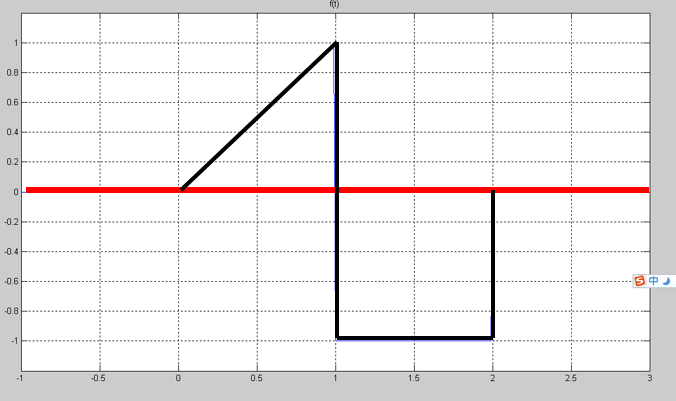
\includegraphics[scale=0.5]{T1.png}
plot:
$$
\begin{aligned}
f(t)+f(t)\\
f(t)\cdot f(t)\\
f(3-4t)\\
f(1-\frac{t}{1.5})\\
f(t)f(3-4t)\\
f'(t)\\
\int f(t)\\
odd-even component of f(t)
\end{aligned}
$$
\subsection{Analysis}
\noindent To generate step function u(t),use \textbf{stepfun()} or \textbf{heaviside()}.\\
For numberical solution, f'(t) must use $lim_{x->\delta x} \frac{f(x+\delta x)-f(x)}{\delta x}$,integration must use sum function.\\
\subsection{Codes and Result}
\textbf{symbolic solution}
\begin{lstlisting}
clear all
close all
syms t;
f=(heaviside(t)-heaviside(t-1))*t-(heaviside(t-1)-heaviside(t-2));
ezplot(f+f,[-1,3]);
line([1,1],[-2,2])
hold on;
grid on;
title('f(t)+f(t)');
\end{lstlisting}
\textbf{Result}\\
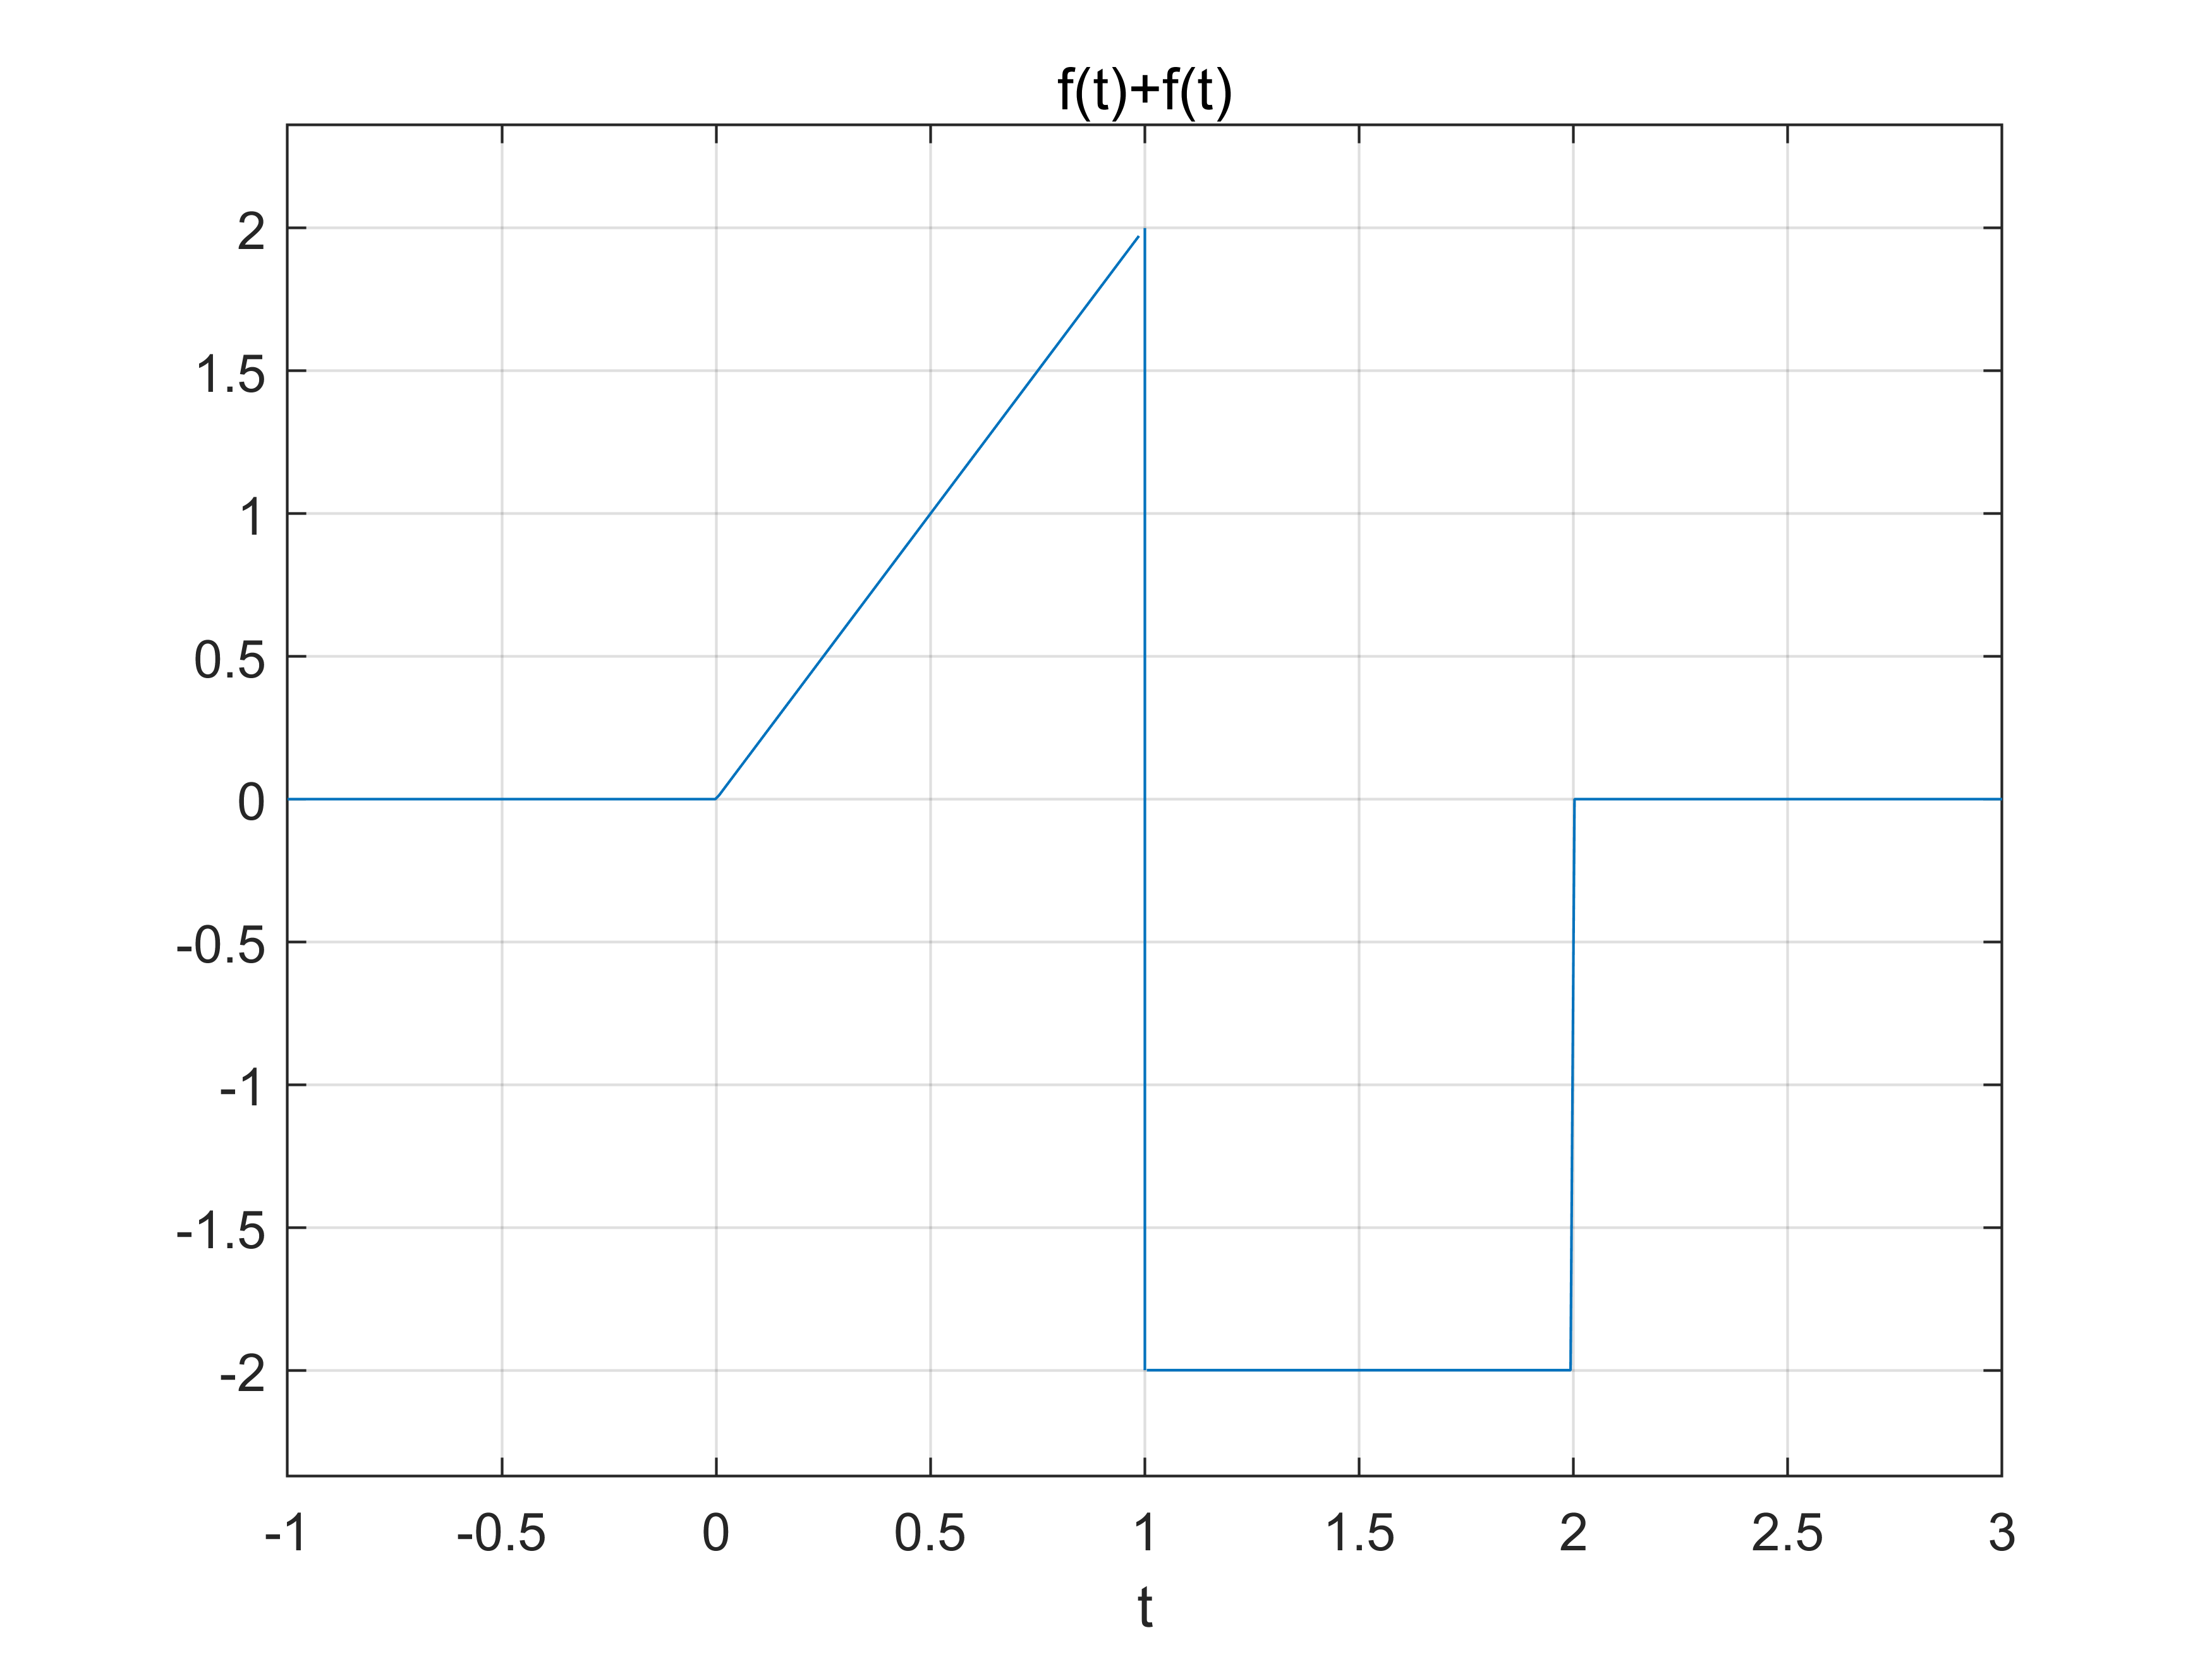
\includegraphics[scale=0.6]{符号法1-1.png}\\
\textbf{Question 2}\\
\begin{lstlisting}
    clear all
    close all
    syms t;
    f=(heaviside(t)-heaviside(t-1))*t-(heaviside(t-1)-heaviside(t-2));
    ezplot(f*f);
    hold on;
    grid on;
    title('f(t)f(t)');
\end{lstlisting}
\textbf{Result}\\
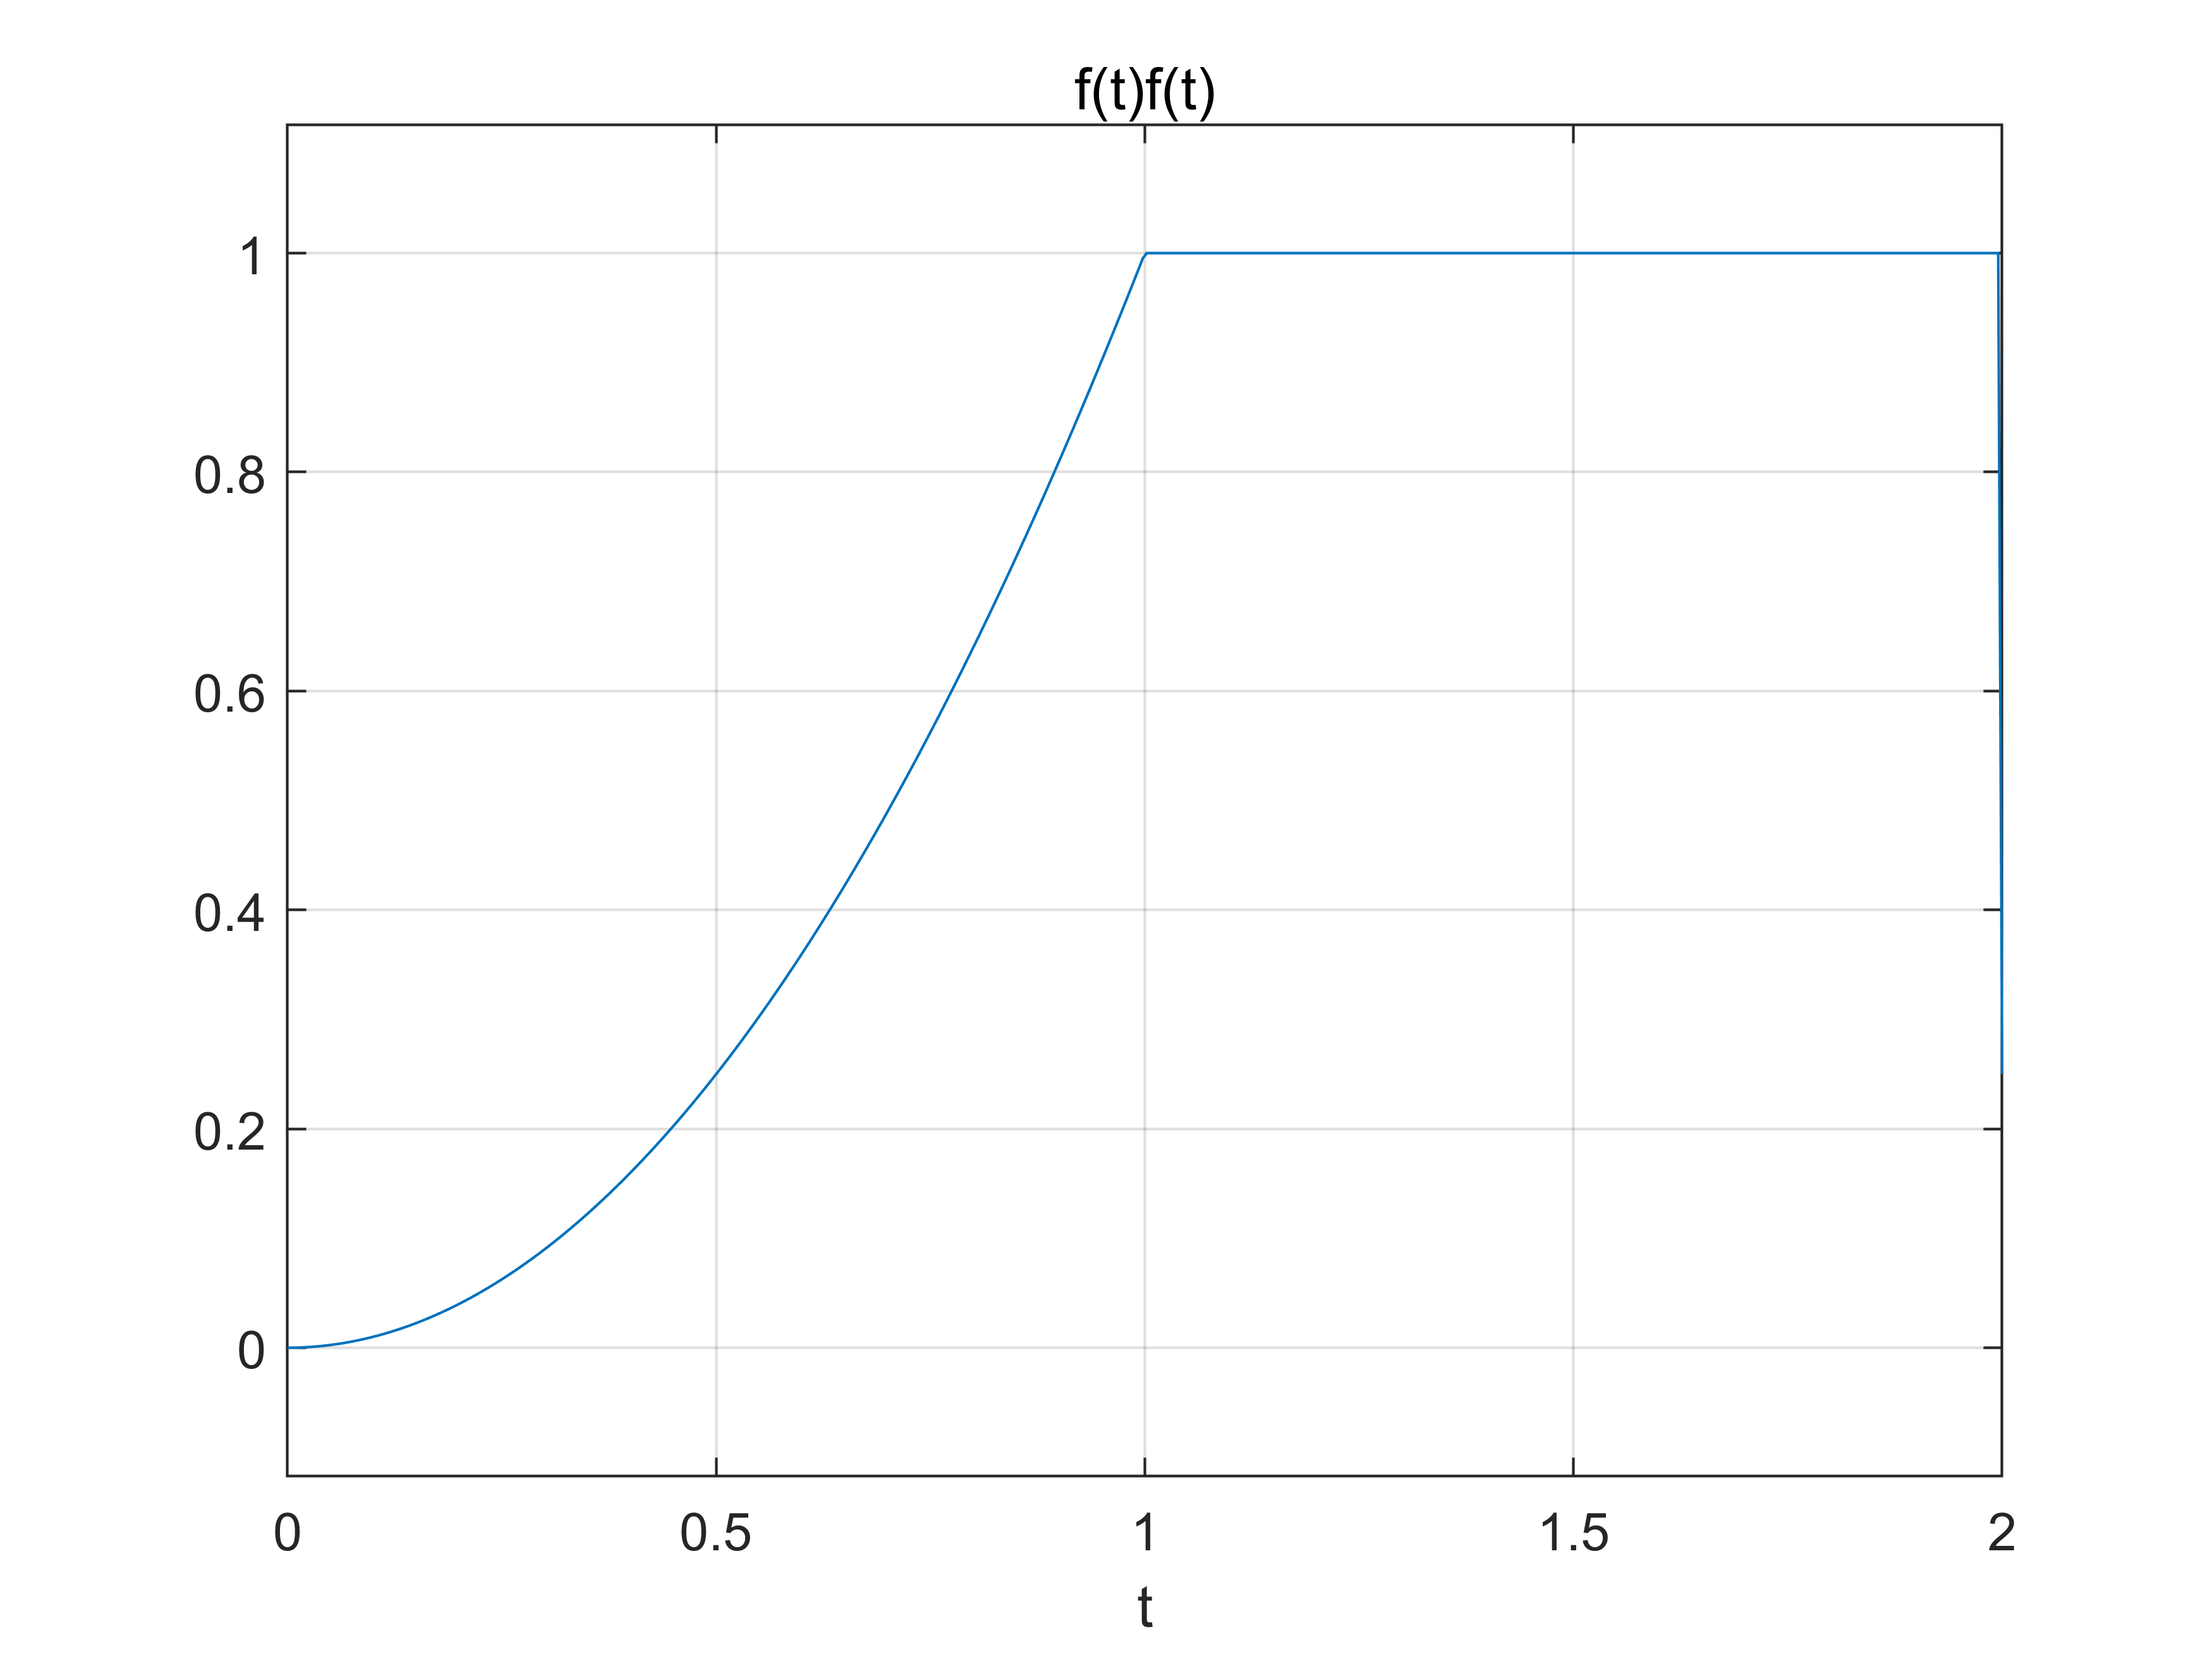
\includegraphics[scale=0.6]{符号1-2.png}\\
\textbf{Question 3}
\begin{lstlisting}
    clear all
    close all
    syms t;
    f=(heaviside(t)-heaviside(t-1))*t-(heaviside(t-1)-heaviside(t-2));
    ezplot(subs(f,t,3-4*t));
    hold on;
    grid on;
    title('f(3-4t)');
\end{lstlisting}
\textbf{Result}\\
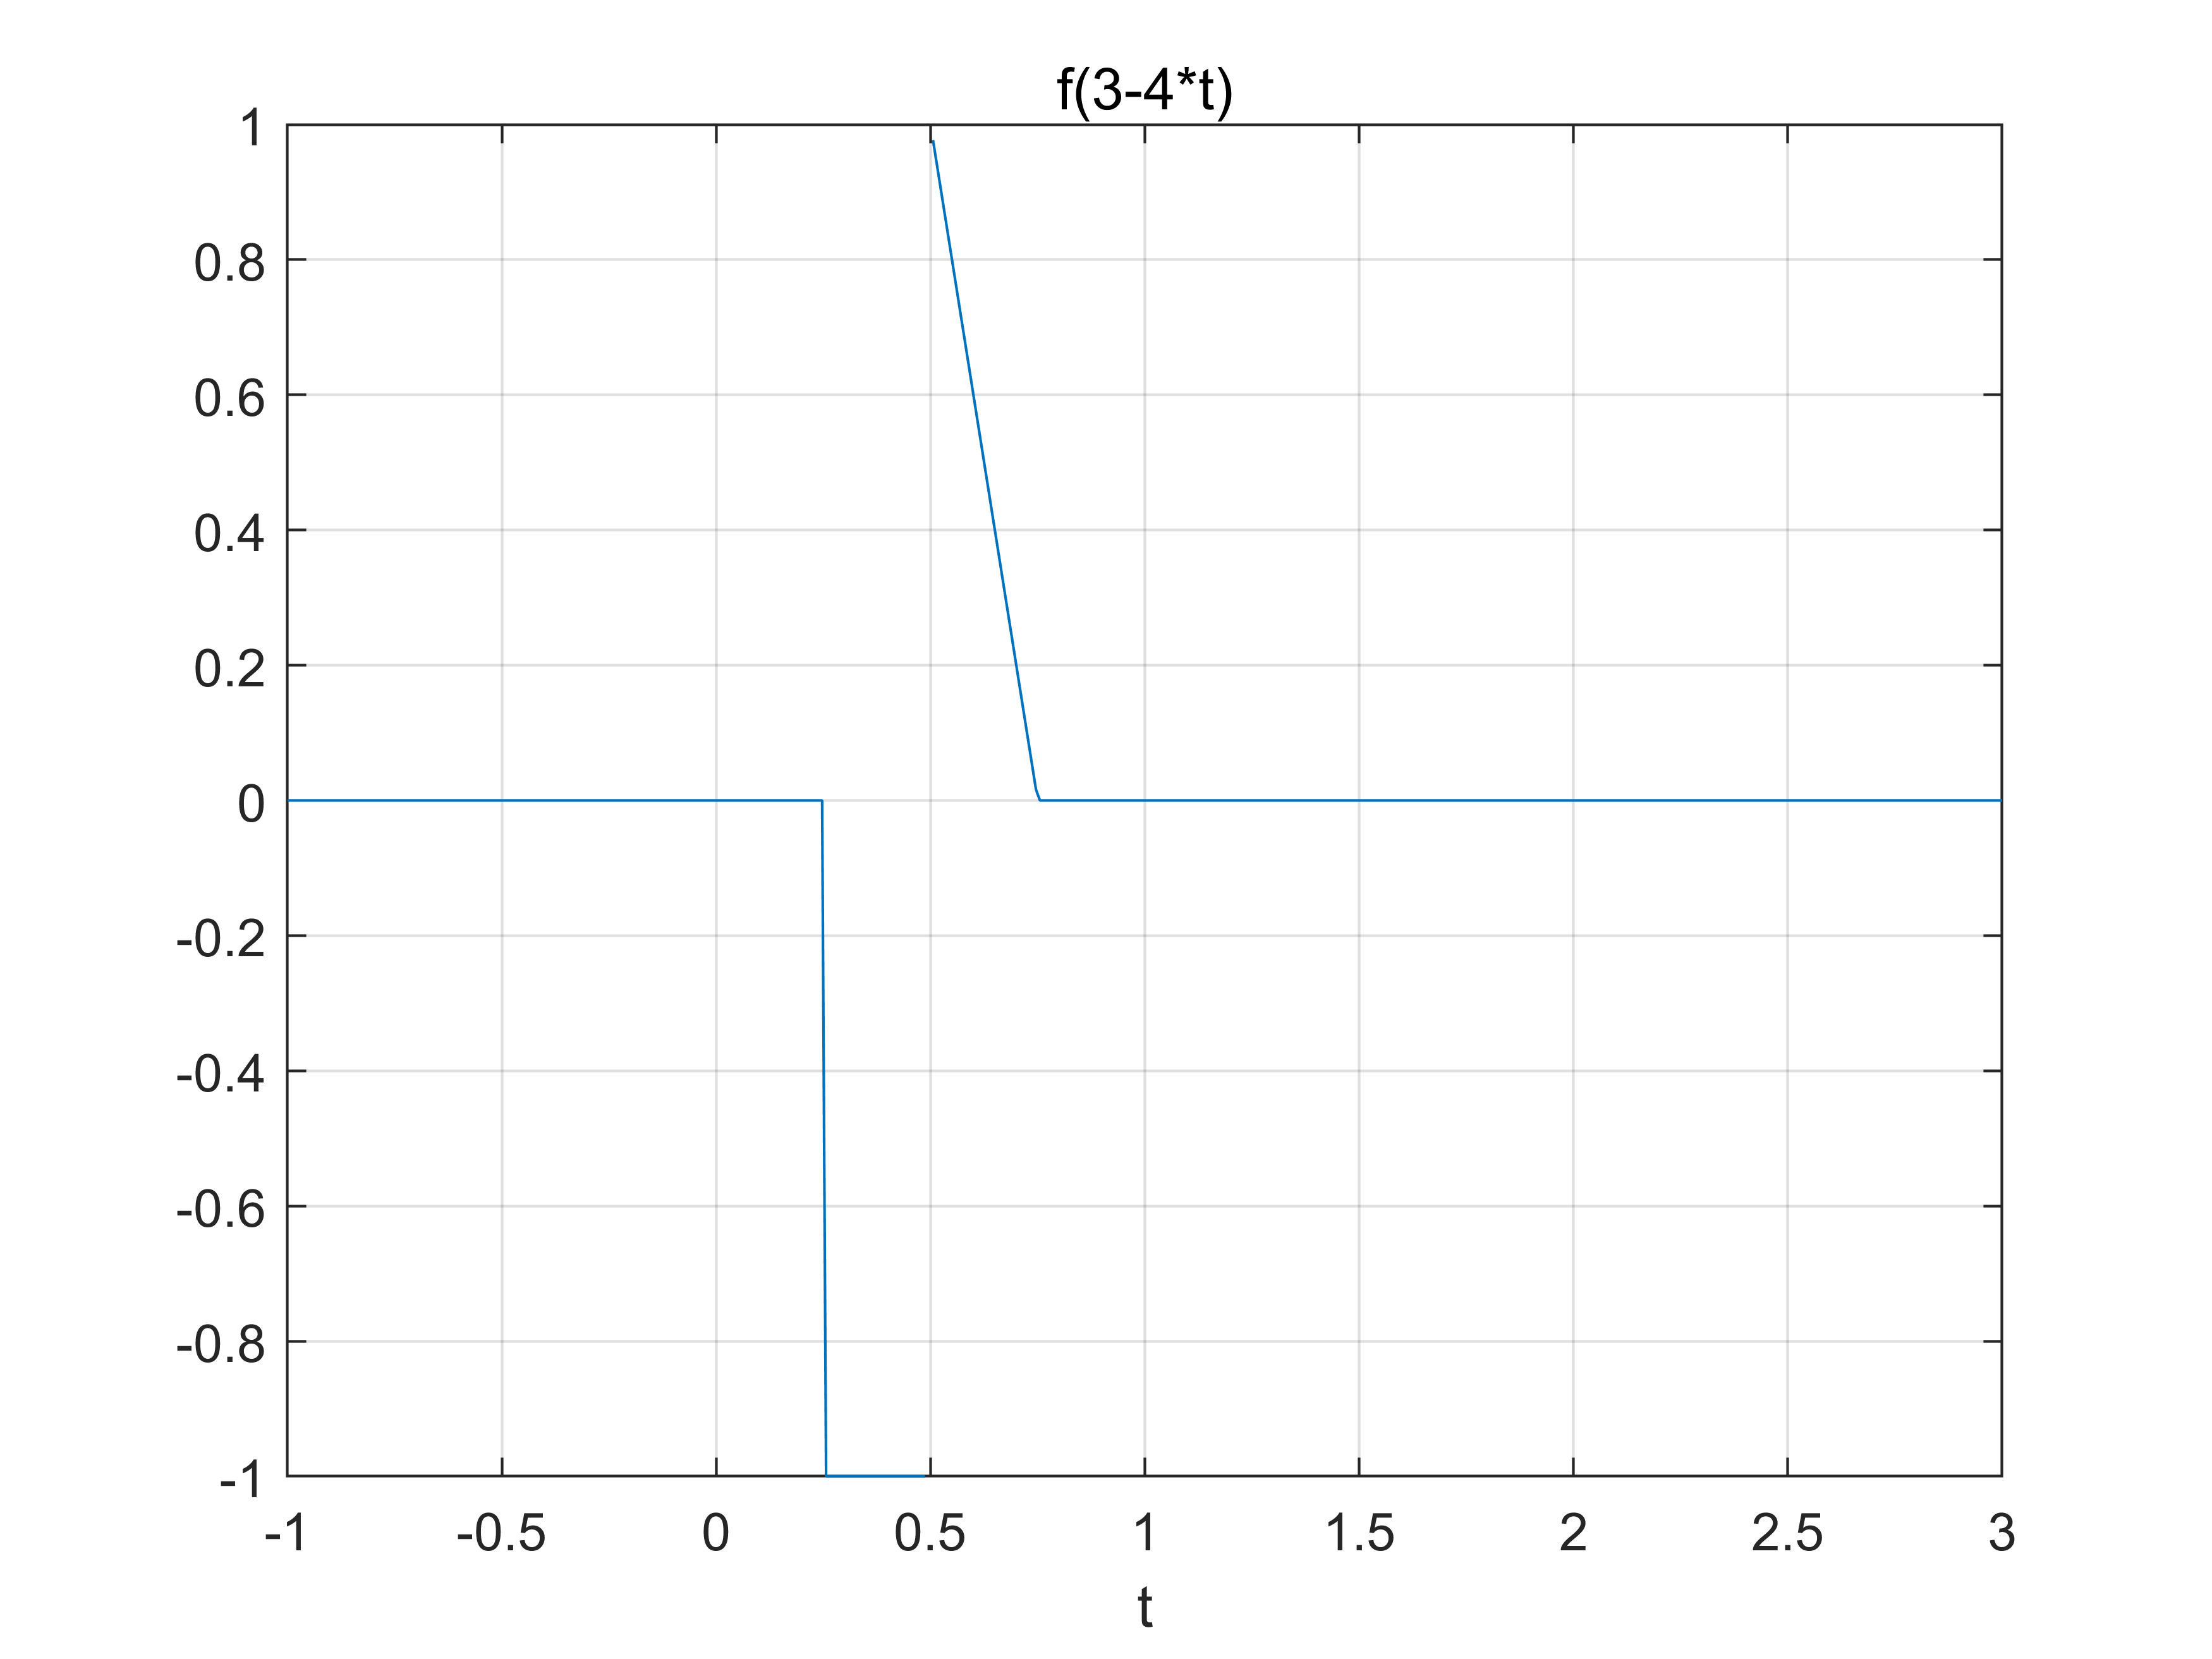
\includegraphics[scale=0.65]{符号1-3.png}\\
\textbf{Question 4}\\
\begin{lstlisting}
    clf;
    syms t;
    f=(heaviside(t)-heaviside(t-1))*t-(heaviside(t-1)-heaviside(t-2));
    ezplot(subs(f,t,1-t/1.5),[-1,3]);
    line([0,0],[-1,1])
    hold on;
    grid on;
    title("$f(1-\frac{t}{1.5})$",'Interpreter','Latex');    
\end{lstlisting}
\textbf{Result}\\
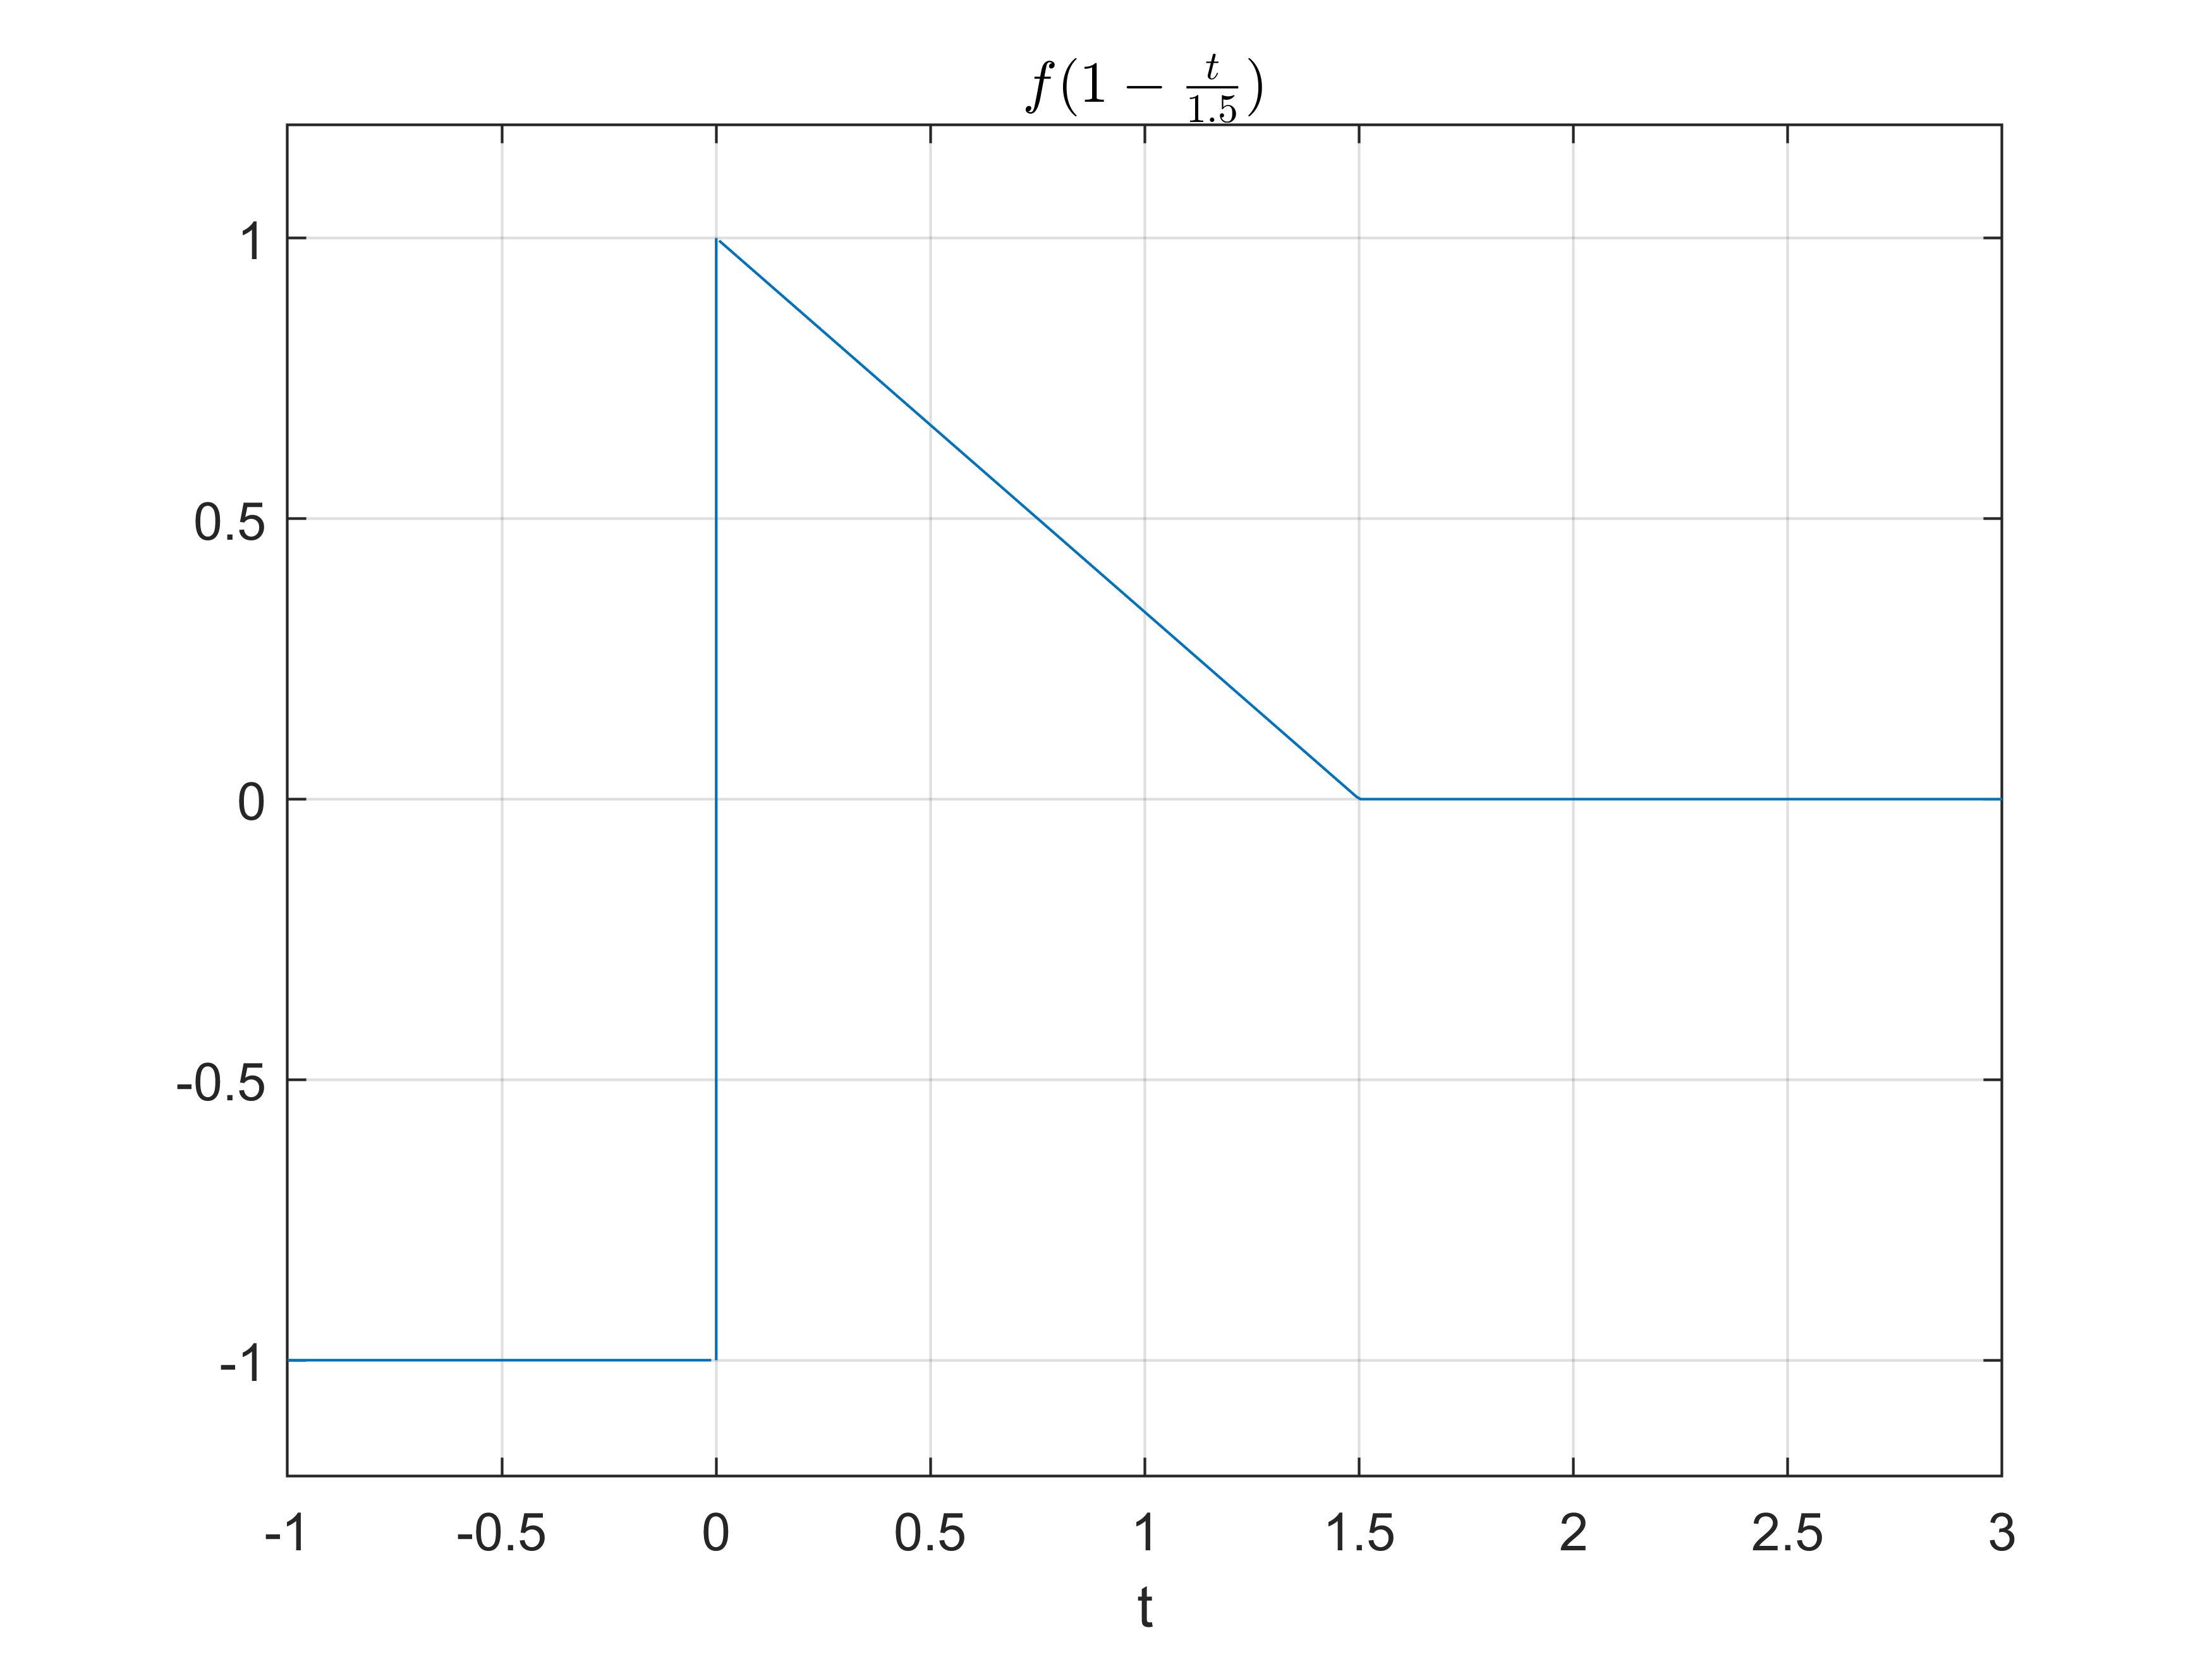
\includegraphics[scale=0.6]{符号1-4.png}\\
\textbf{Question 5}\\
\begin{lstlisting}
clear all
close all
syms t;
f=(heaviside(t)-heaviside(t-1))*t-(heaviside(t-1)-heaviside(t-2));
ezplot(f*subs(f,t,3-4*t));
line([0.5,0.5],[-0.5,0.5])
hold on;
grid on;
title('f(t)f(3-4t)');
\end{lstlisting}
\textbf{Result}\\
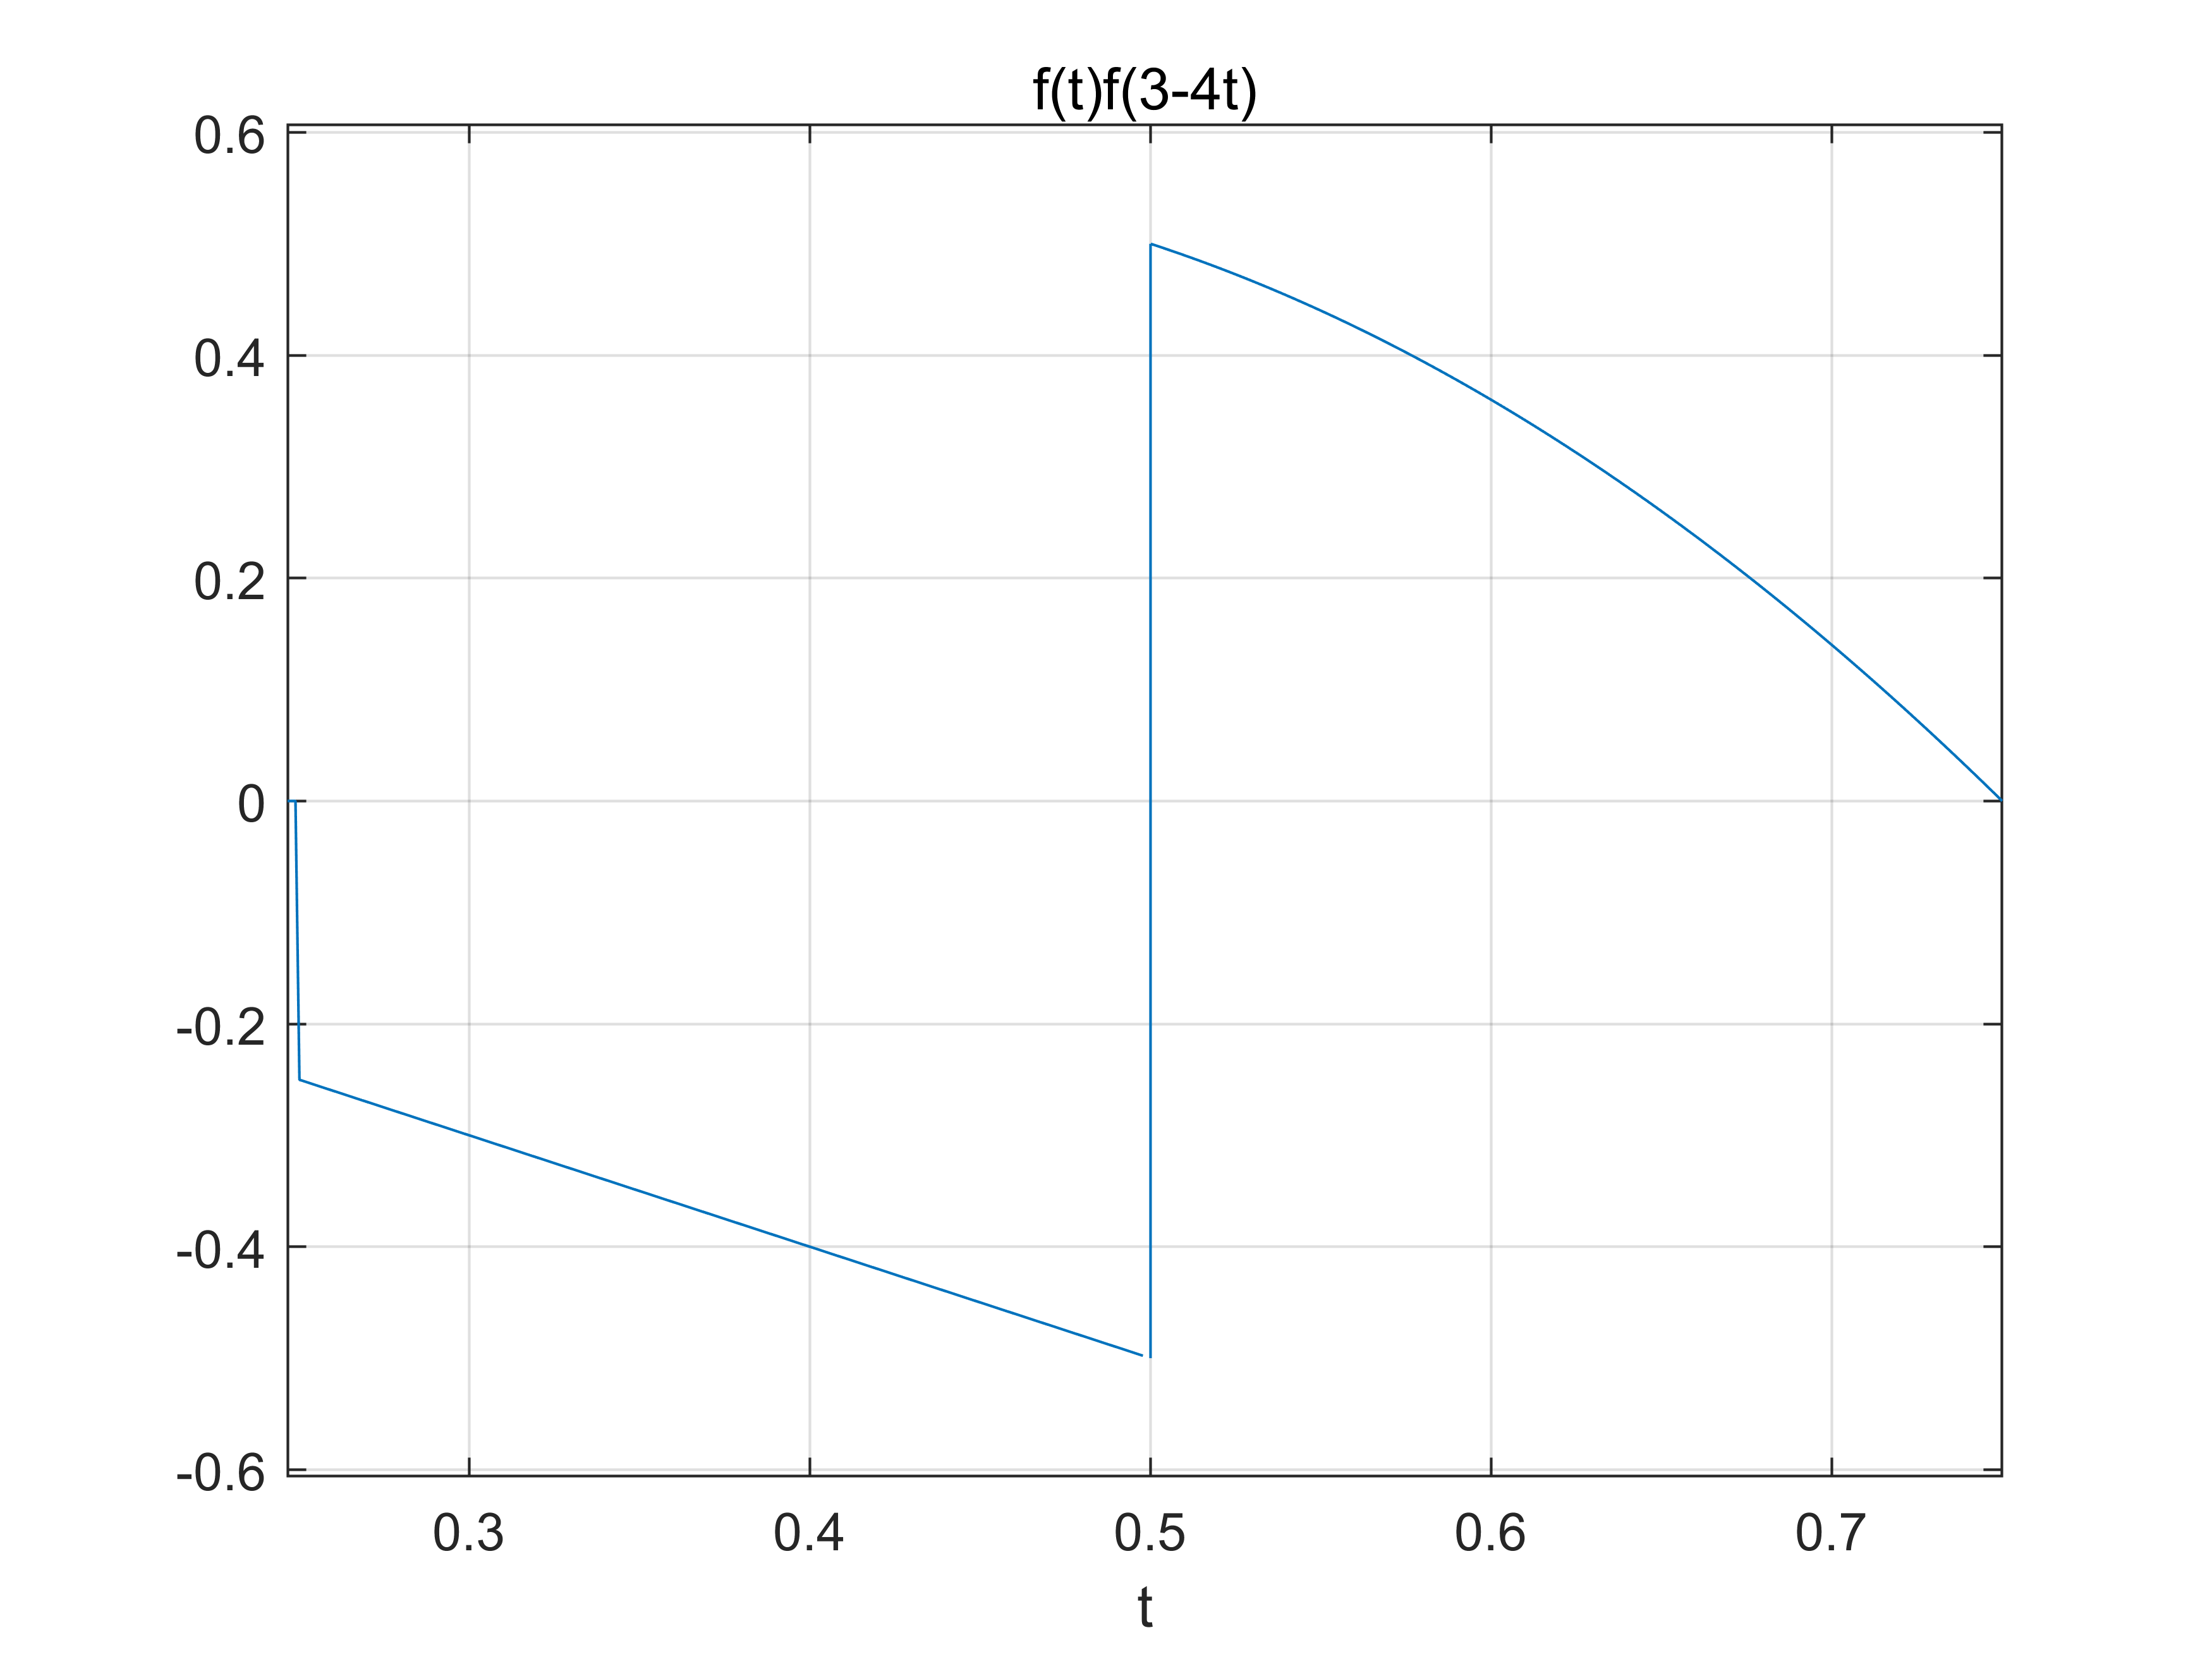
\includegraphics[scale=0.6]{符号1-5.png}\\
\textbf{Question 6}\\
\begin{lstlisting}
    clear all
    close all
    syms t;
    f=(heaviside(t)-heaviside(t-1))*t-(heaviside(t-1)-heaviside(t-2));
    ezplot(diff(f,t));
    line([0.5,0.5],[-0.5,0.5])
    hold on;
    grid on;
    title("f(t)'");
\end{lstlisting}
\textbf{Result}\\
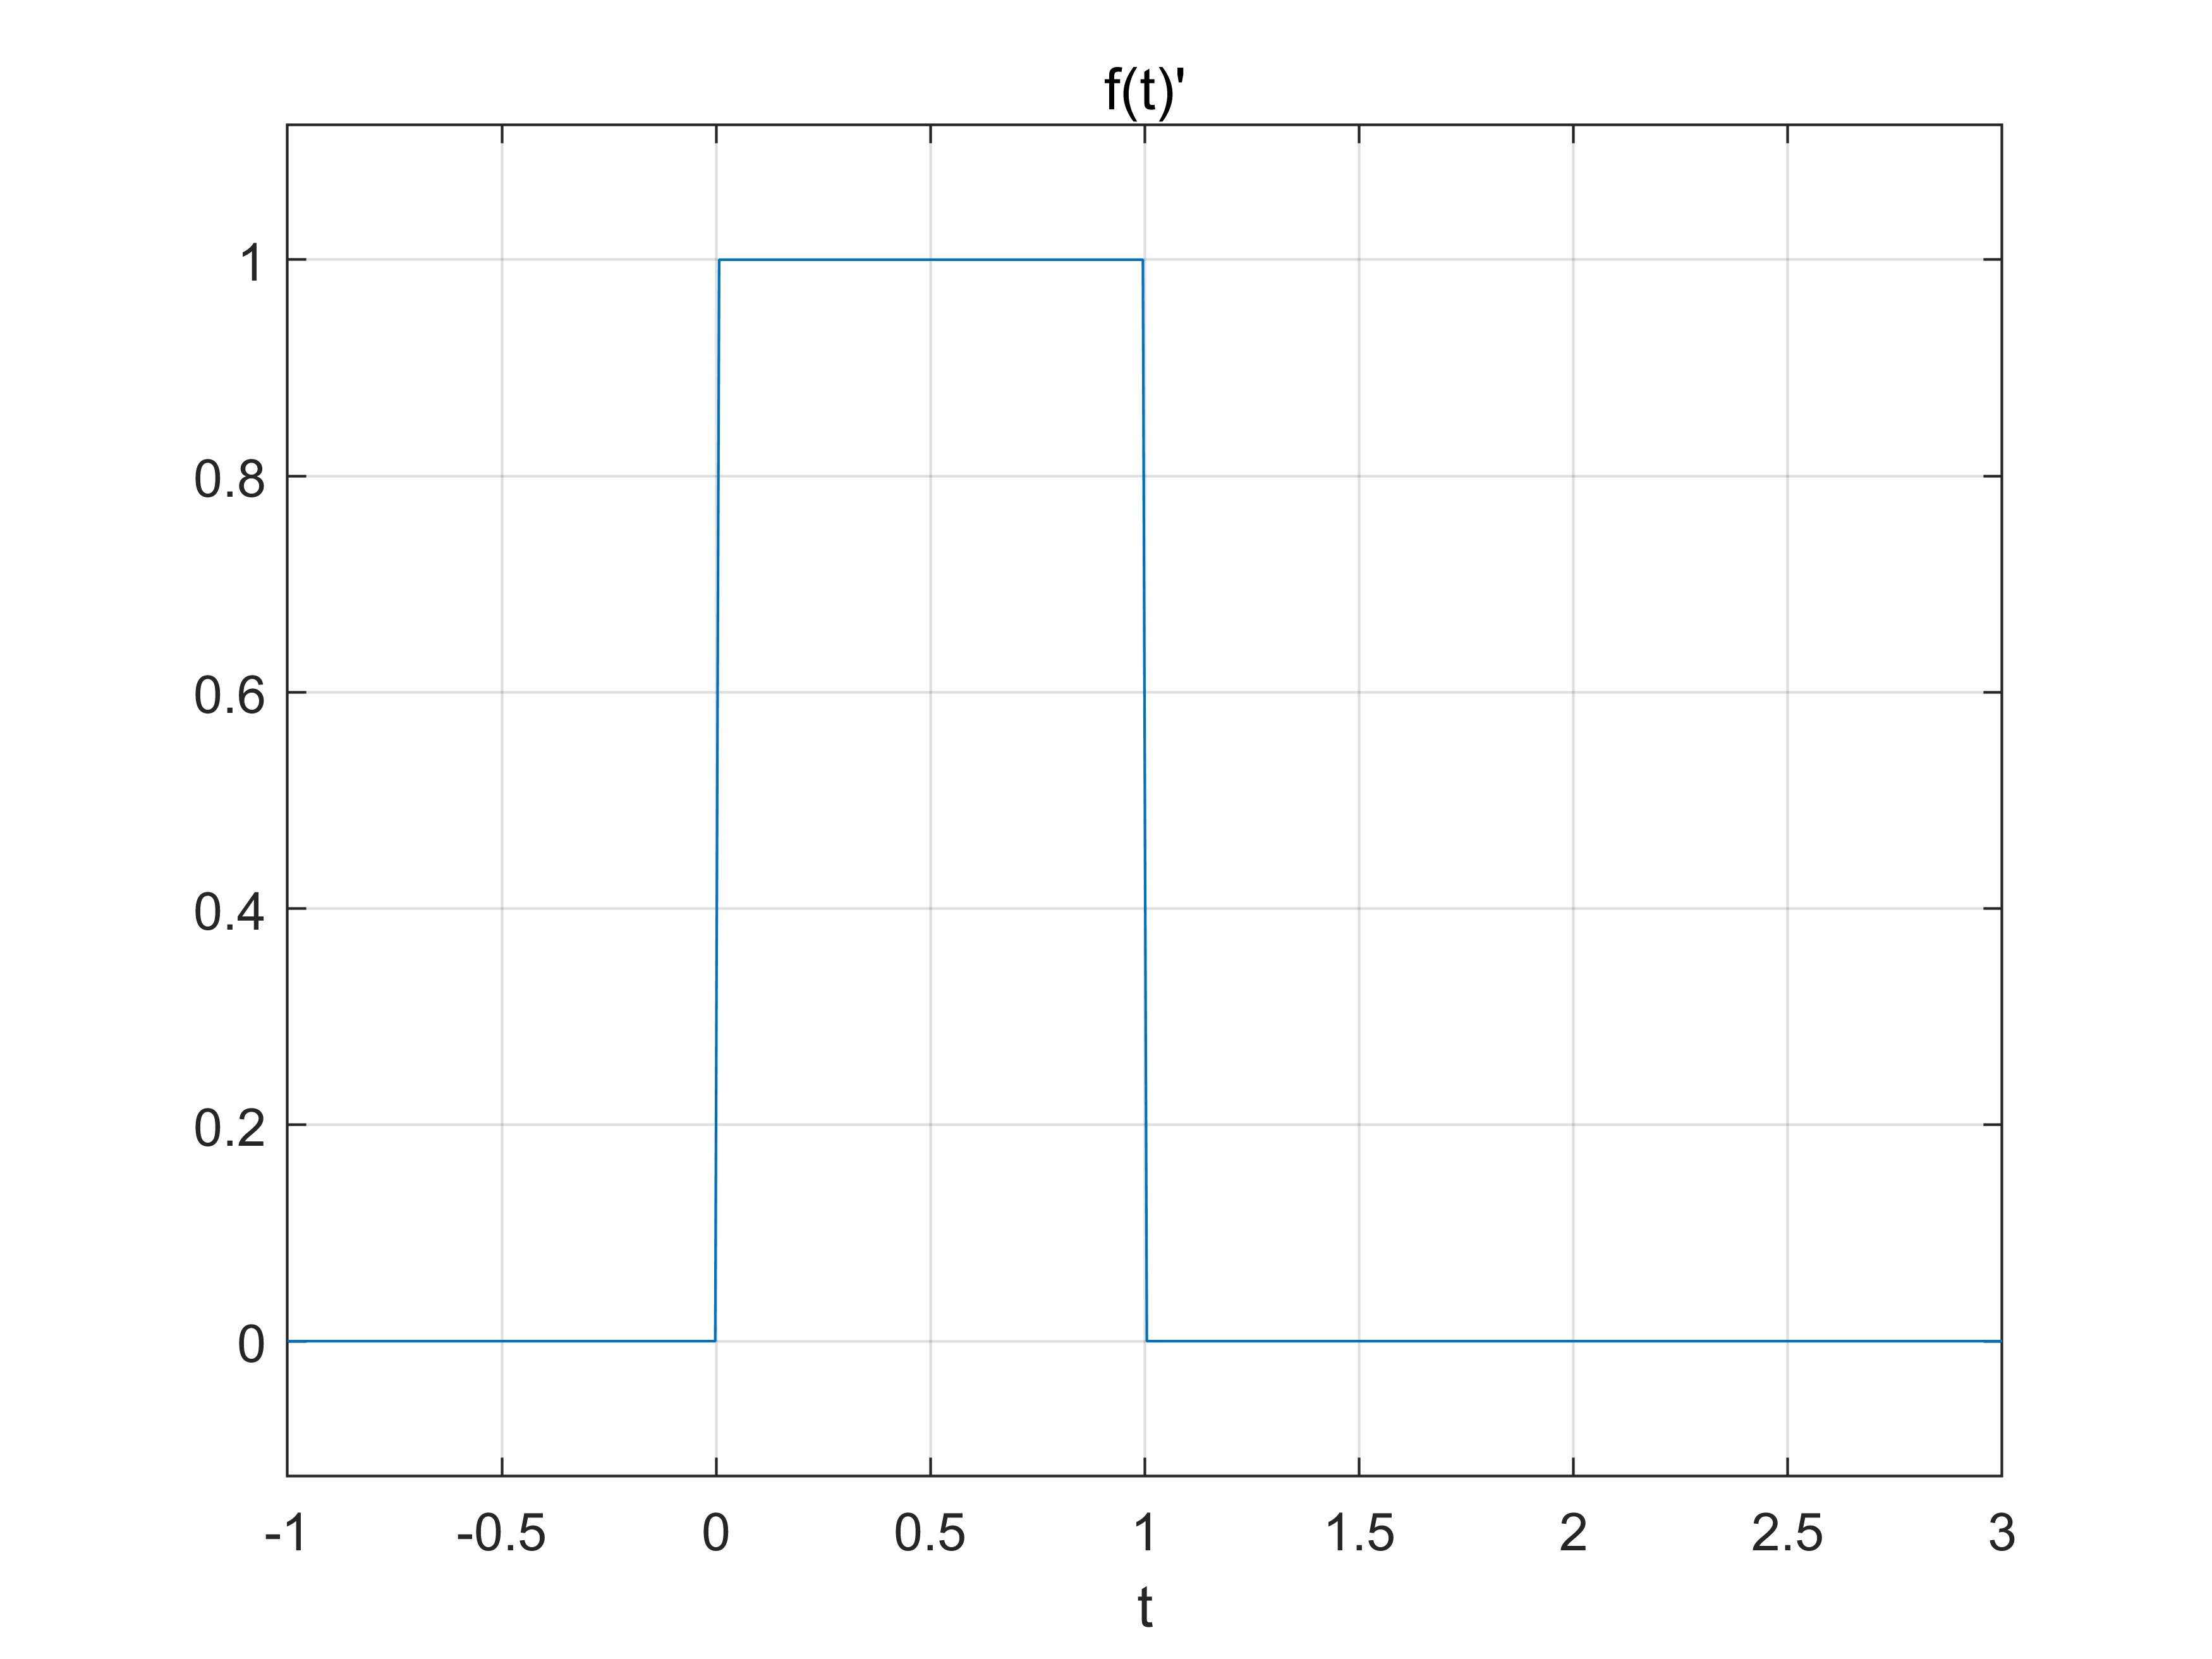
\includegraphics[scale=0.6]{符号1-6.png}\\
\textbf{Question 7}\\
\begin{lstlisting}
    clf;
    syms t;
    f=(heaviside(t)-heaviside(t-1))*t-(heaviside(t-1)-heaviside(t-2));
    ezplot(int(f,t,-inf,t),[-1,3]);
    %line([],[])
    hold on;
    grid on;
    title("$\int f(t)$",'Interpreter','Latex');
\end{lstlisting}
\textbf{Result}\\
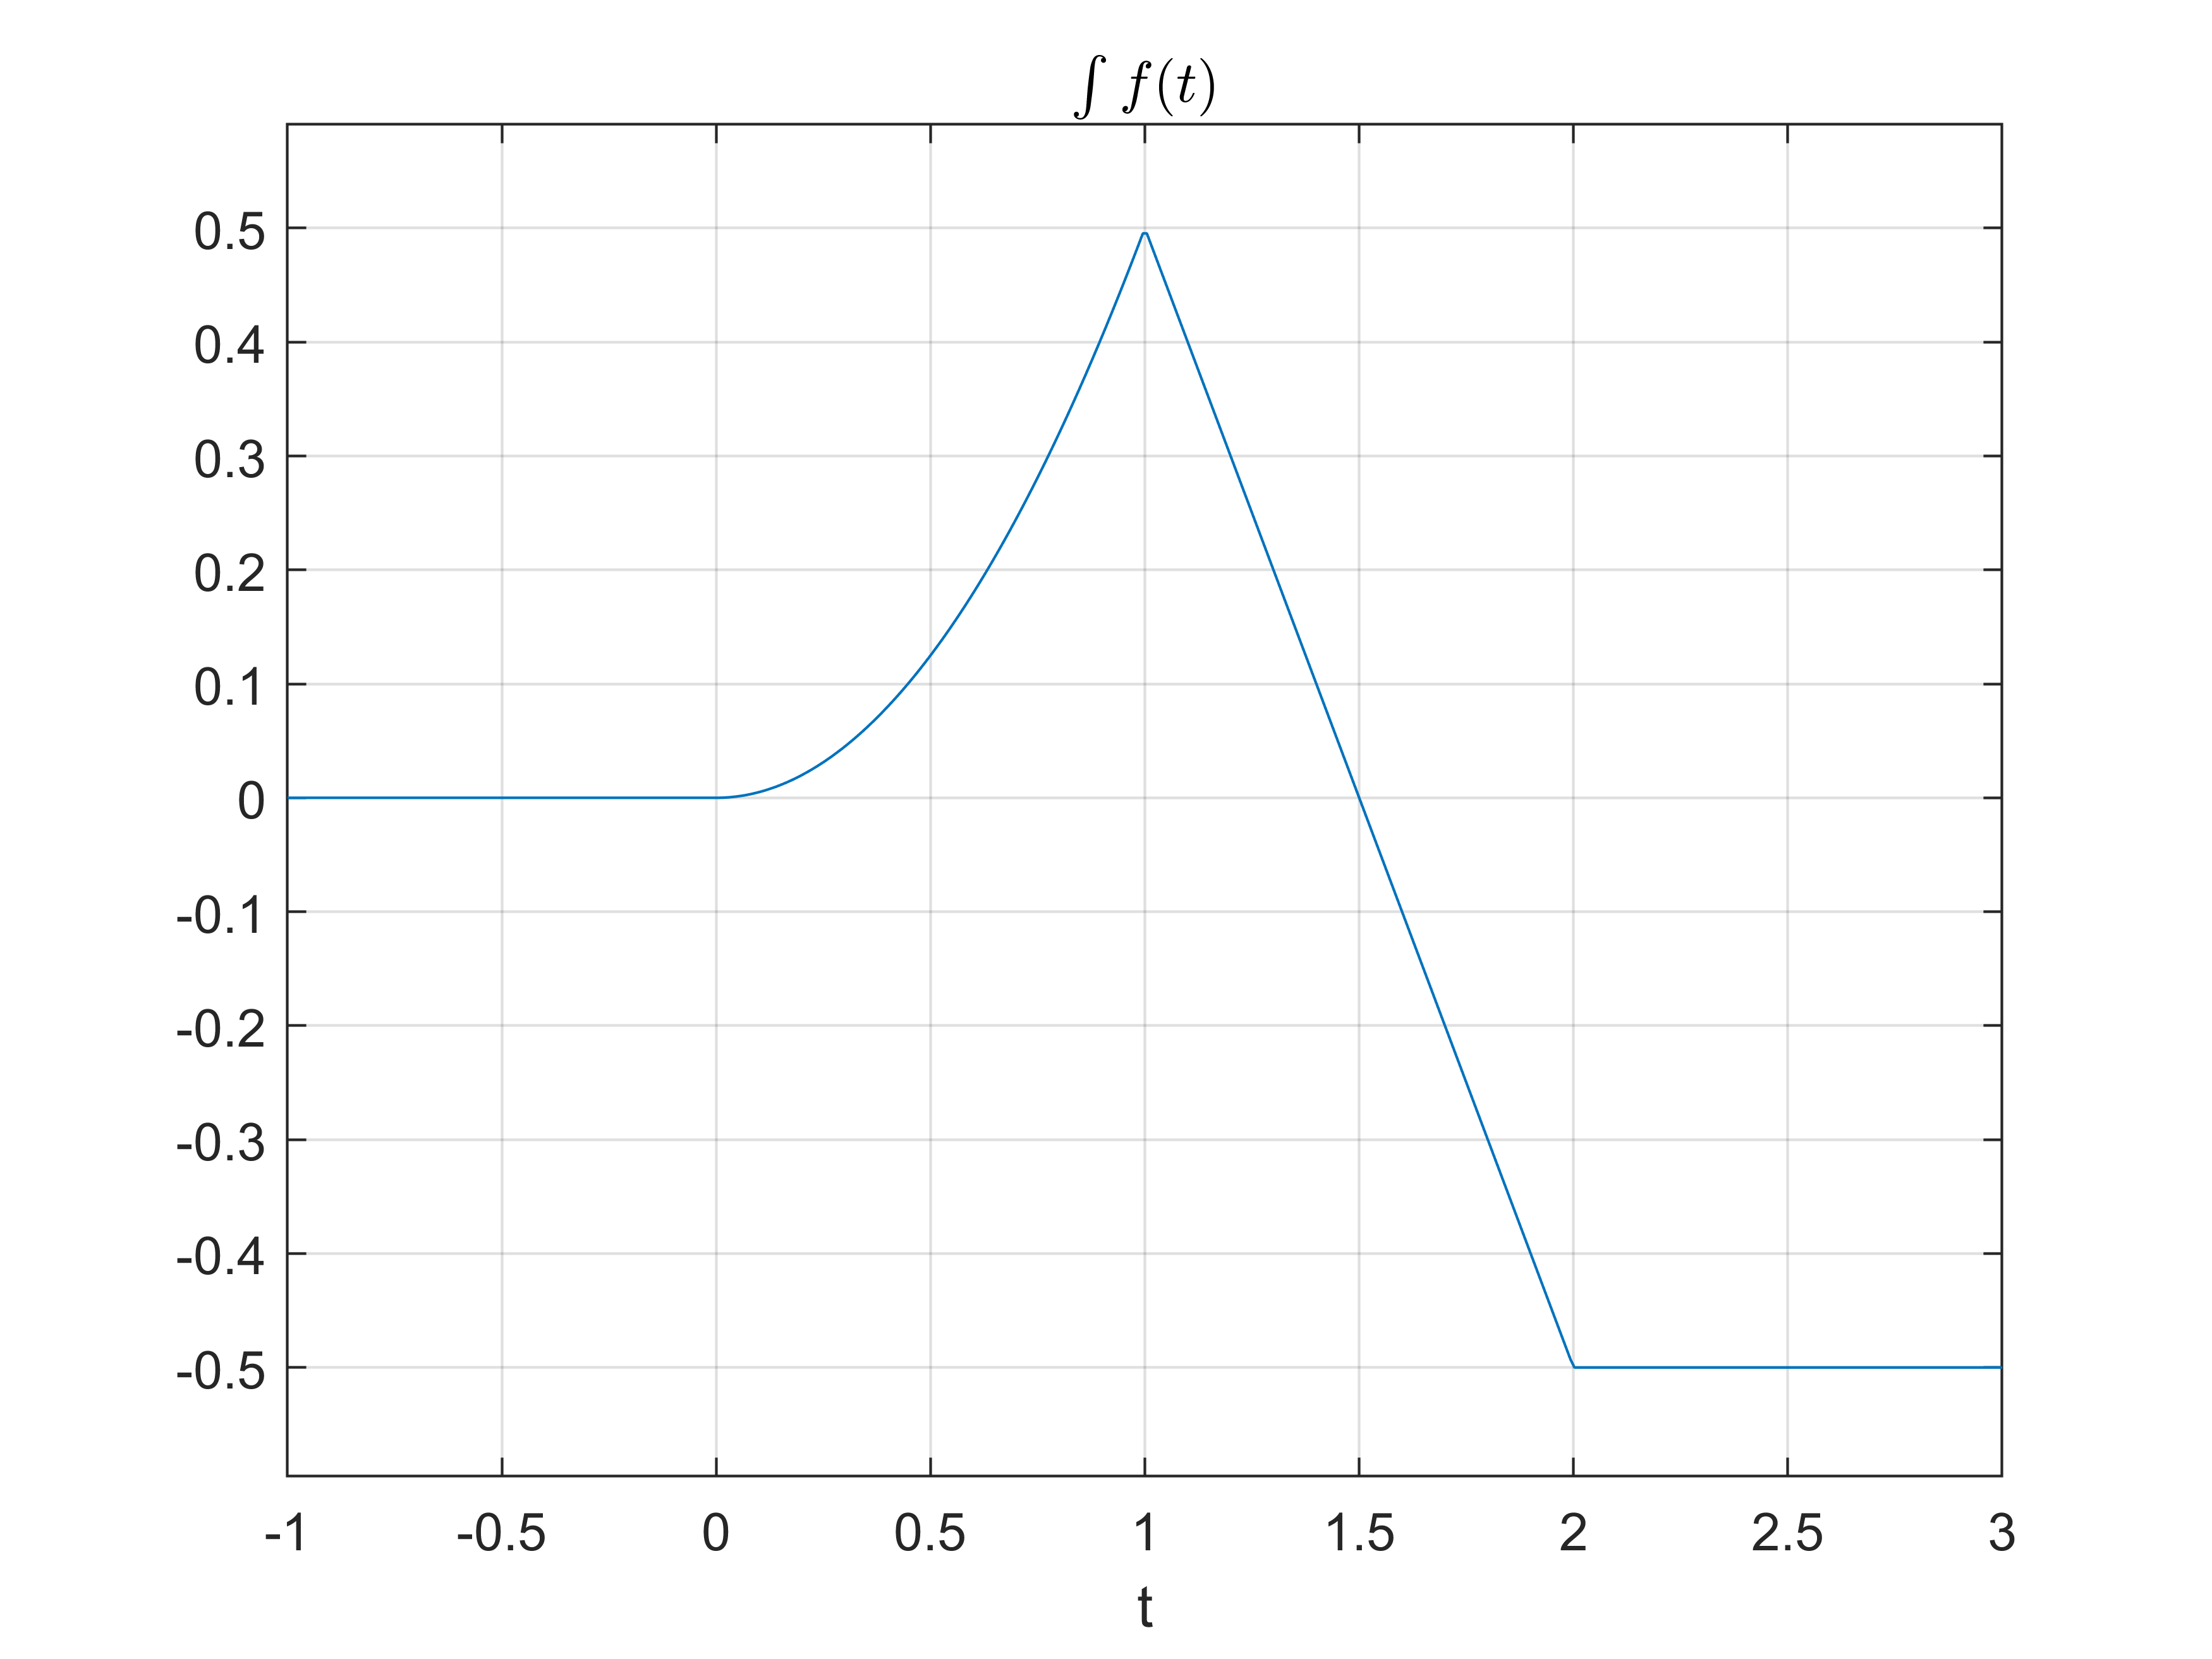
\includegraphics[scale=0.6]{符号1-7.png}\\
\textbf{Question 8}\\
\begin{lstlisting}
    clf;
    syms t;
    f=(heaviside(t)-heaviside(t-1))*t-(heaviside(t-1)-heaviside(t-2));
    fe=(f+subs(f,t,-t))/2;
    fo=(f-subs(f,t,-t))/2;
    subplot(1,2,1);
    ezplot(fe,[-3,3]);
    hold on;
    line([-1,-1],[-0.5,0.5]);
    line([1,1],[-0.5,0.5]);
    grid on;
    title('fe(t)')
    subplot(1,2,2);
    ezplot(fo,[-3,3]);
    hold on;
    line([1,1],[-0.5,0.5]);
    line([-1,-1],[-0.5,0.5]);
    title('fo(t)')
    grid on;
\end{lstlisting}
\textbf{Result}\\
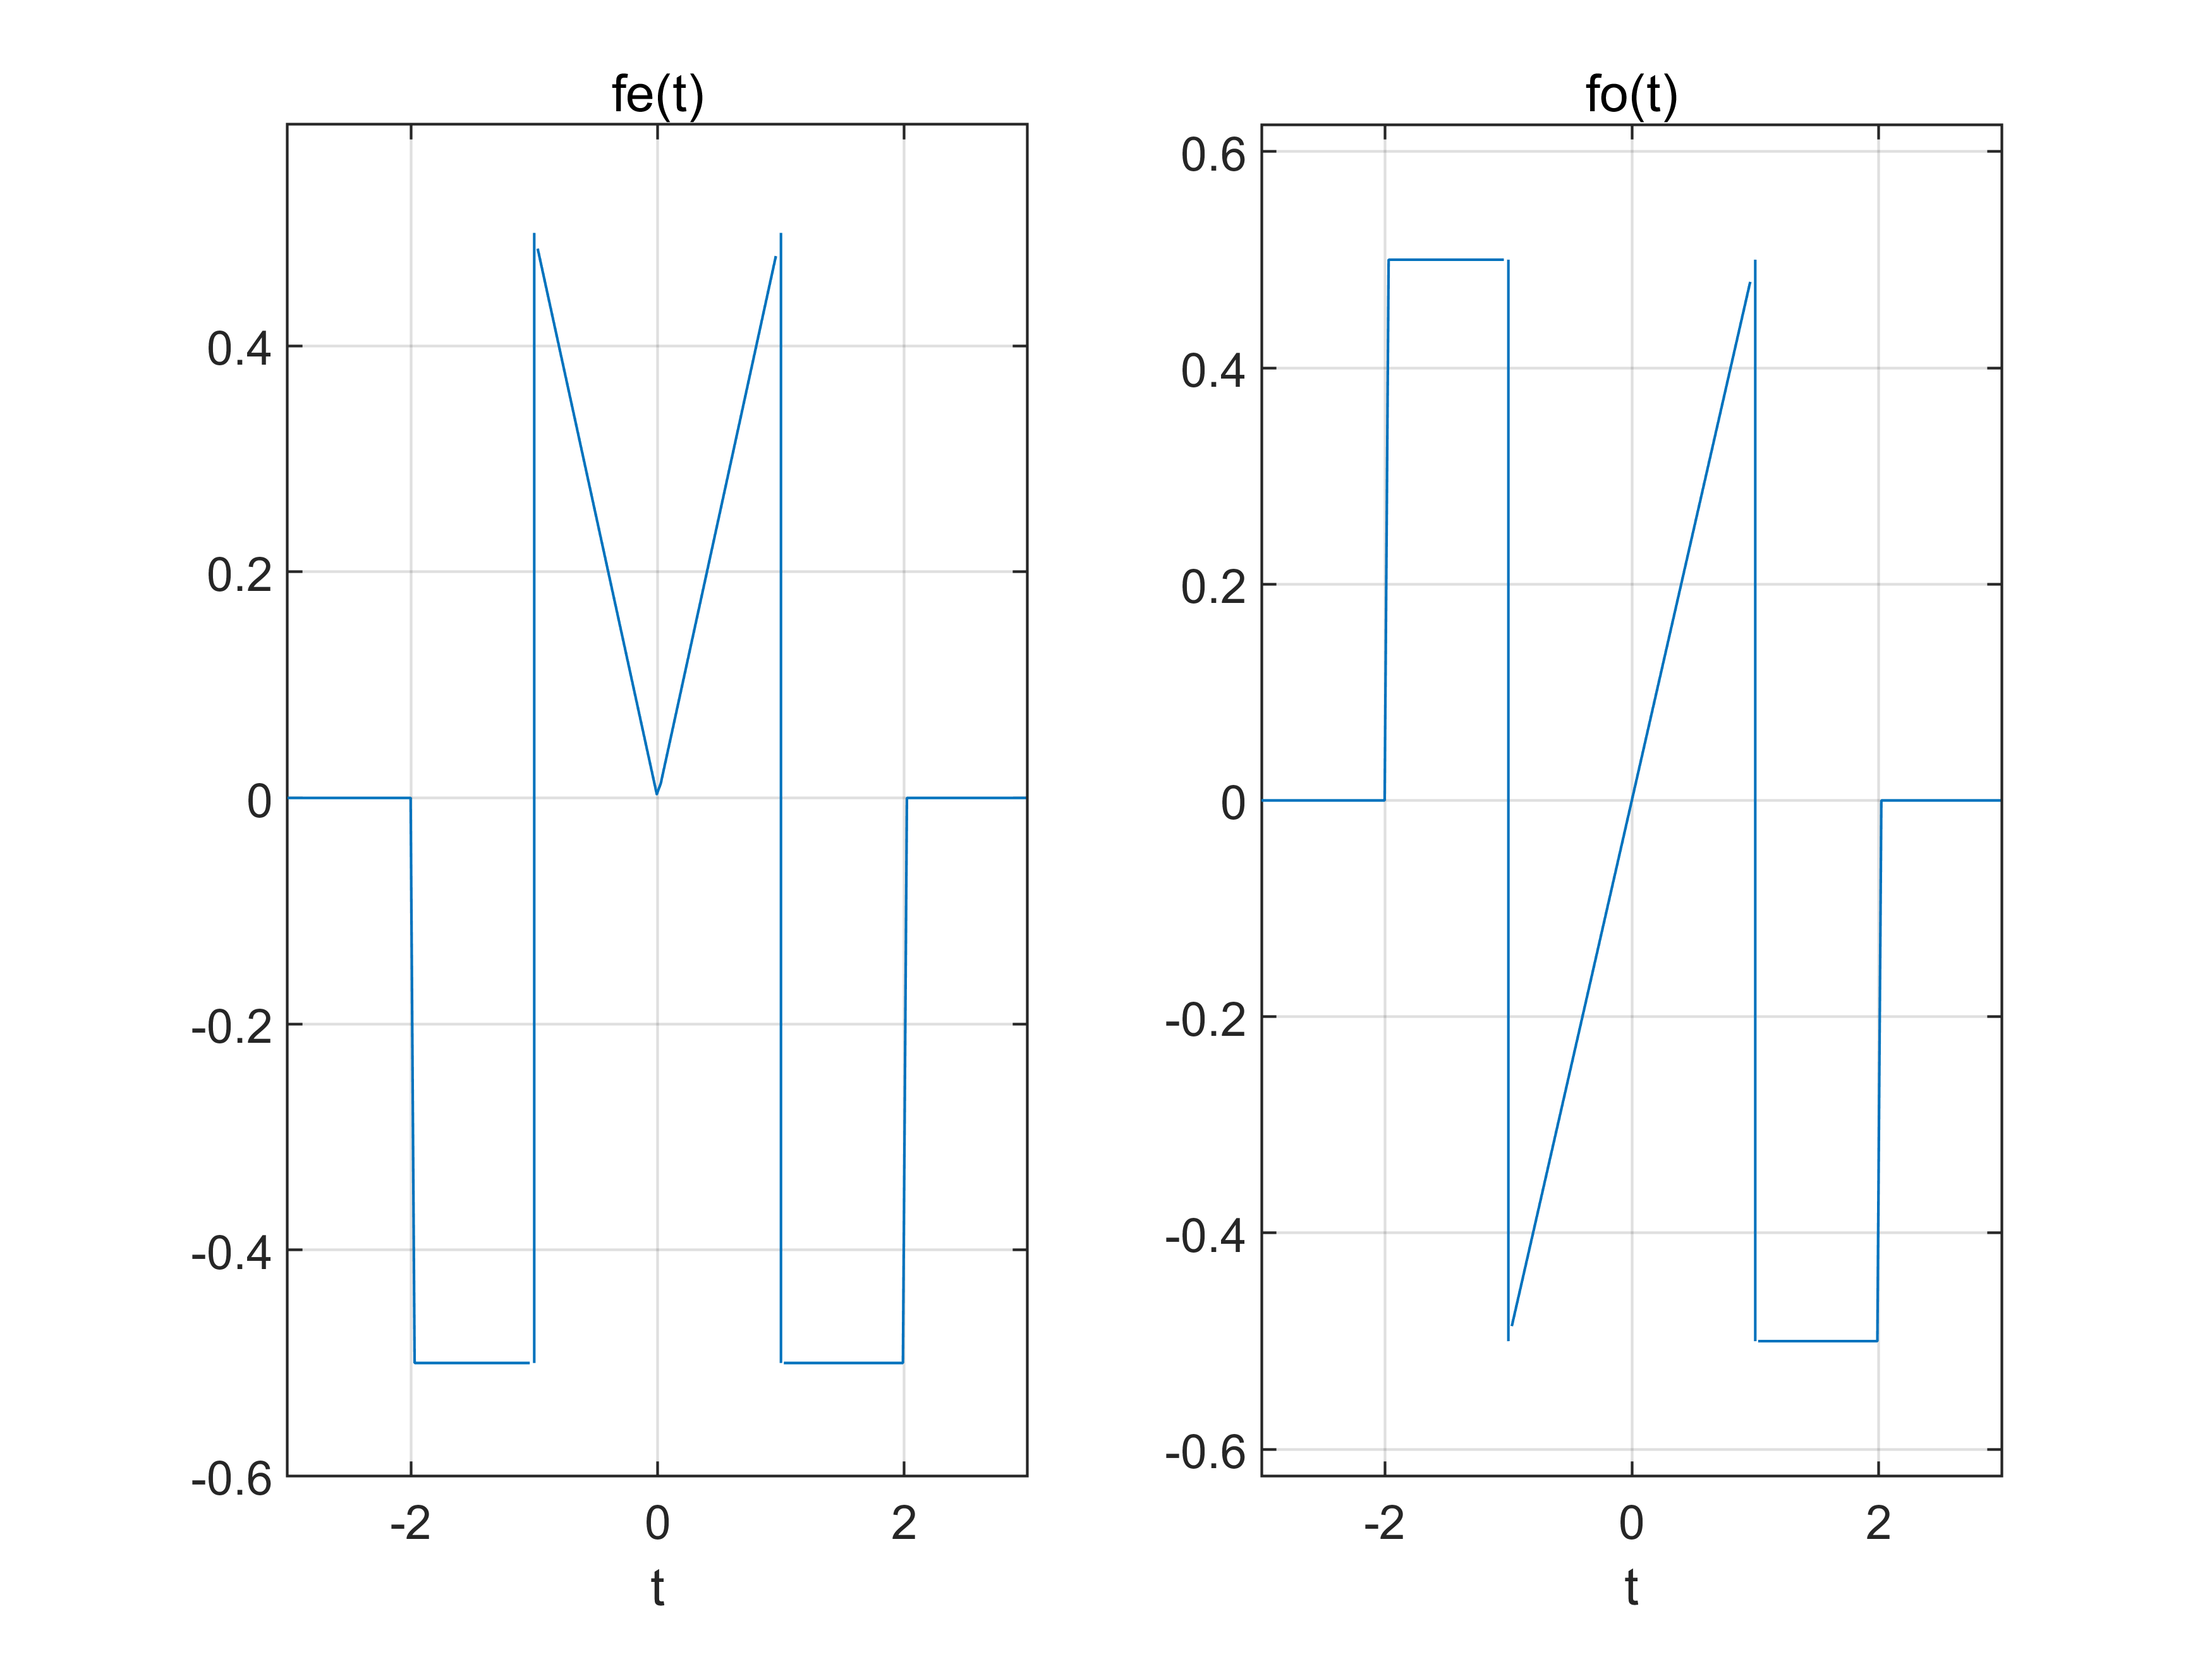
\includegraphics[scale=0.6]{符号1-8.png}\\
\textbf{Numberical method}\\
\begin{lstlisting}
1、
clear all
close all
t=-3:0.01:3;
f=(heaviside(t)-heaviside(t-1)).*t-(heaviside(t-1)-heaviside(t-2));
plot(t,f);
axis([-3,3,-2,2])
line([1,1],[-2,2])
hold on;
grid on;
title('f(t)+f(t)');
2
clear all
close all
t=-3:0.01:3;
f=(heaviside(t)-heaviside(t-1))*t-(heaviside(t-1)-heaviside(t-2));
plot(t,f.*f);
hold on;
grid on;
title('f(t)f(t)');
3、
clear all
close all
t;
f=(heaviside(t)-heaviside(t-1))*t-(heaviside(t-1)-heaviside(t-2));
ezplot(subs(f,t,3-4*t));
hold on;
grid on;
title('f(3-4t)');
4、
clf;
t=-3:0.01:3;
f=(heaviside(3-4*t)-heaviside(3-4*t-1)).*t-(heaviside(3-4*t-1)-heaviside(3-4*t-2));
plot(t,f);
hold on;
grid on;
title("$f(1-\frac{t}{1.5})$",'Interpreter','Latex');
5、
clear all
close all
t=-3:0.01:3;
f=(heaviside(t)-heaviside(t-1)).*t-(heaviside(t-1)-heaviside(t-2)).*(heaviside(3-4*t)-heaviside(3-4*t-1)).*t-(heaviside(3-4*t-1)-heaviside(3-4*t-2));
plot(t,f);
hold on;
line([0.5,0.5],[-0.5,0.5])
grid on;
title('f(t)f(3-4t)');
6、
t=-3:0.01:3;
f=(heaviside(t)-heaviside(t-1)).*t-(heaviside(t-1)-heaviside(t-2));
for i=-3:0.01:3
    if i~=-3 
        y(round((i+3)/0.01)+1)=(f(round((i+3)/0.01)+1)-f(round((i+3)/0.01)))/0.01;
    else y(1)=(f(1)-0)/0.01;
    end
    
end 
plot(t,y);
hold on;
grid on;
title("f(t)'");
7、
clf;
t=-3:0.01:3;
f=(heaviside(t)-heaviside(t-1)).*t-(heaviside(t-1)-heaviside(t-2));
for i=-3:0.01:3
    f1(round((i+3)/0.01+1))=sum(f(1:round((i+3)/0.01)+1))*0.01;
end
plot(t,f1);
%line([],[])
hold on;
grid on;
title("$\int f(t)$",'Interpreter','Latex');
8、
clf;
t=-3:0.01:3;
f=(heaviside(t)-heaviside(t-1)).*t-(heaviside(t-1)-heaviside(t-2));
fe=(f+fliplr(f))/2;
fo=(f-fliplr(f))/2;
subplot(1,2,1);
plot(t,fe);
hold on;
axis([-3,3,-1,1])
grid on;
title('fe(t)')
subplot(1,2,2);
plot(t,fo);
hold on;
%line([1,1],[-0.5,0.5]);
%line([-1,-1],[-0.5,0.5]);
title('fo(t)')
axis([-3,3,-1,1]);
grid on;
\end{lstlisting}
\begin{center}
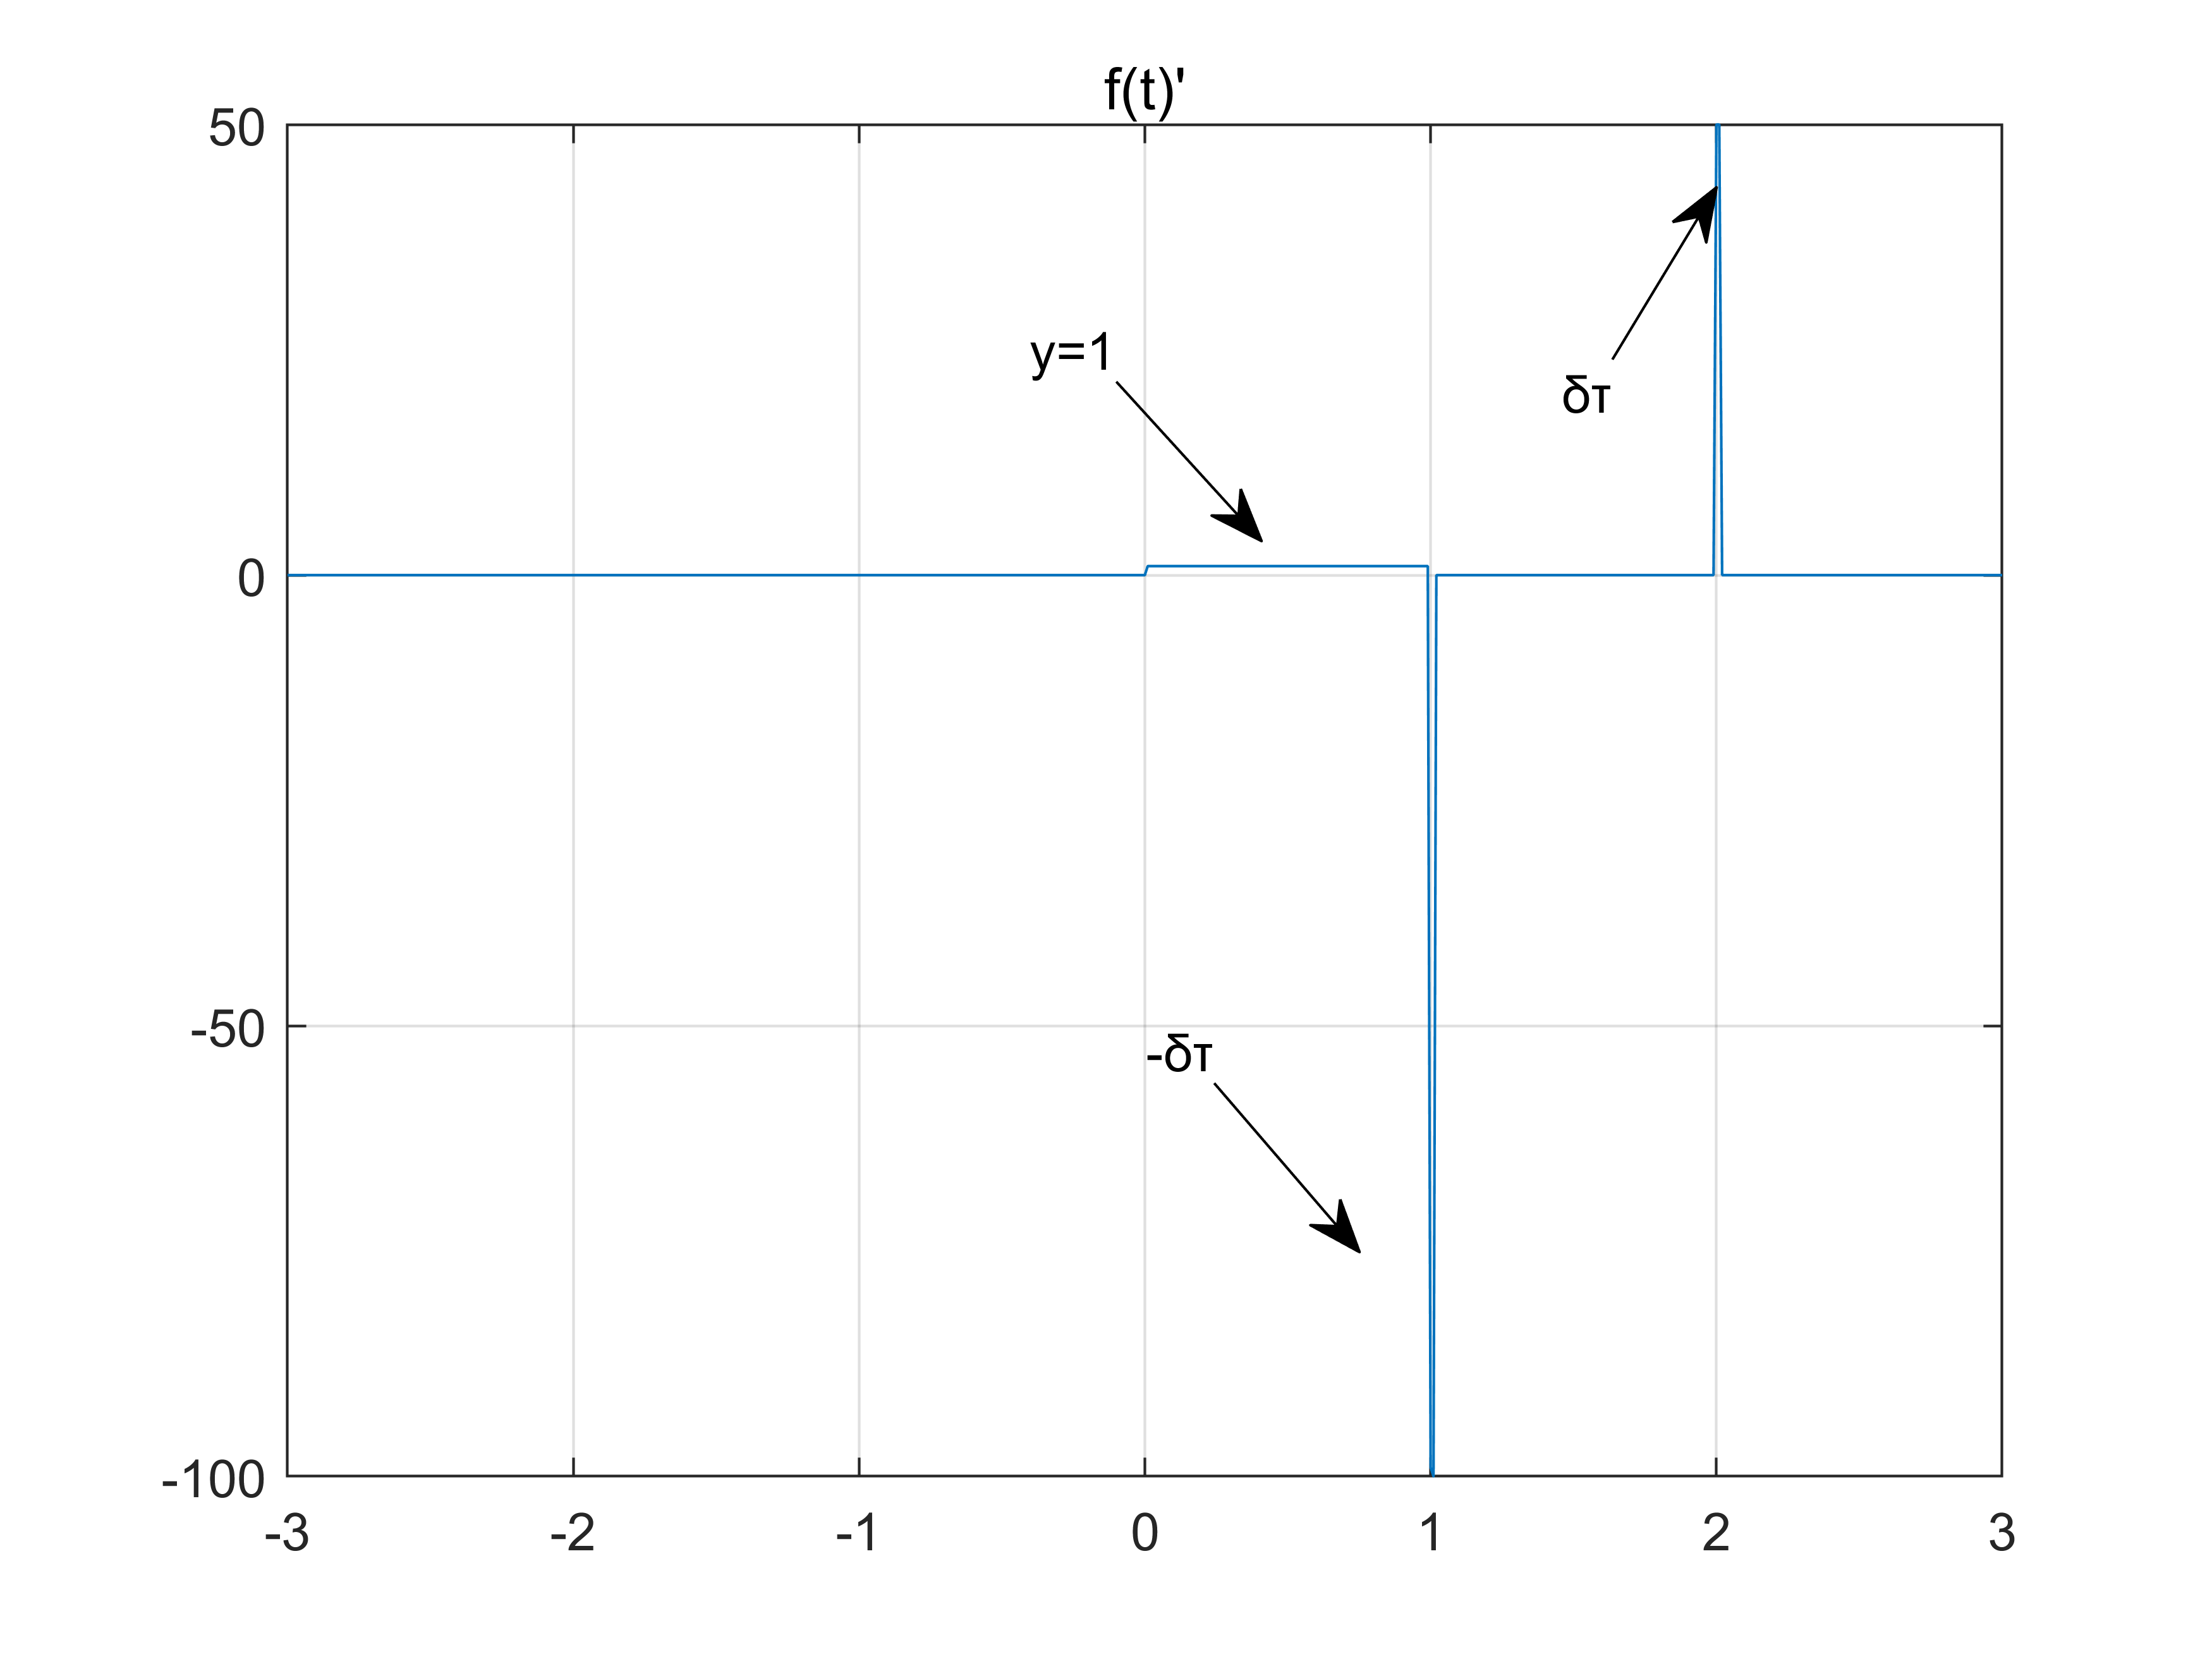
\includegraphics[scale=0.6]{1-6数值.png}\\
numberical solution for T6 shows $\delta t$ on the figure.
\end{center}
\section{Plot f}
\subsection{Description}
$f=\frac{sin(\pi t)}{t}$,plot figures as follow.
\begin{center}
$$
\begin{aligned}
2f(t-1)~~~~~f(2t)\\
-f(0.25t)~~f(1-0.5t)
\end{aligned}
$$
\end{center}
\subsection{Anaylsis}
\noindent use function \textbf{subplot(),plot,ezplot() }.
\subsection{Code and Result}
\begin{lstlisting}
%Numberical method
t=-10:0.01:10;
subplot(2,2,1);
f=2*sinc(t-1)*pi;
plot(t,f);
hold on;
grid on;
title('2f(t-1)');
subplot(2,2,2);
f=sinc(2*t)*pi;
plot(t,f);
hold on;
grid on;
title('f(2t)');
subplot(2,2,3);
f=-sinc(0.25*t)*pi;
plot(t,f)
hold on;
grid on;
title('-f(0.25t)');
subplot(2,2,4);
f=sinc(1-0.5*t)*pi;
plot(t,f);
hold on;
grid on;
title('f(1-0.5t)')         
\end{lstlisting}
\textbf{symbolic solution}
\begin{lstlisting}
    f=sinc(t)*pi;
    subplot(2,2,1);
    ezplot(2*subs(f,t,t-1));
    hold on;
    grid on;
    title('2f(t-1)');
    subplot(2,2,2);
    ezplot(2*subs(f,t,2*t));
    hold on;
    grid on;
    title('f(2t)');
    subplot(2,2,3);
    ezplot(-subs(f,t,0.25*t));
    hold on;
    grid on;
    title('-f(0.25t)');
    subplot(2,2,4);
    ezplot(subs(f,t,1-0.5*t));
    hold on;
    grid on;
    title('f(1-0.5t)')    
\end{lstlisting}
\textbf{Result}\\
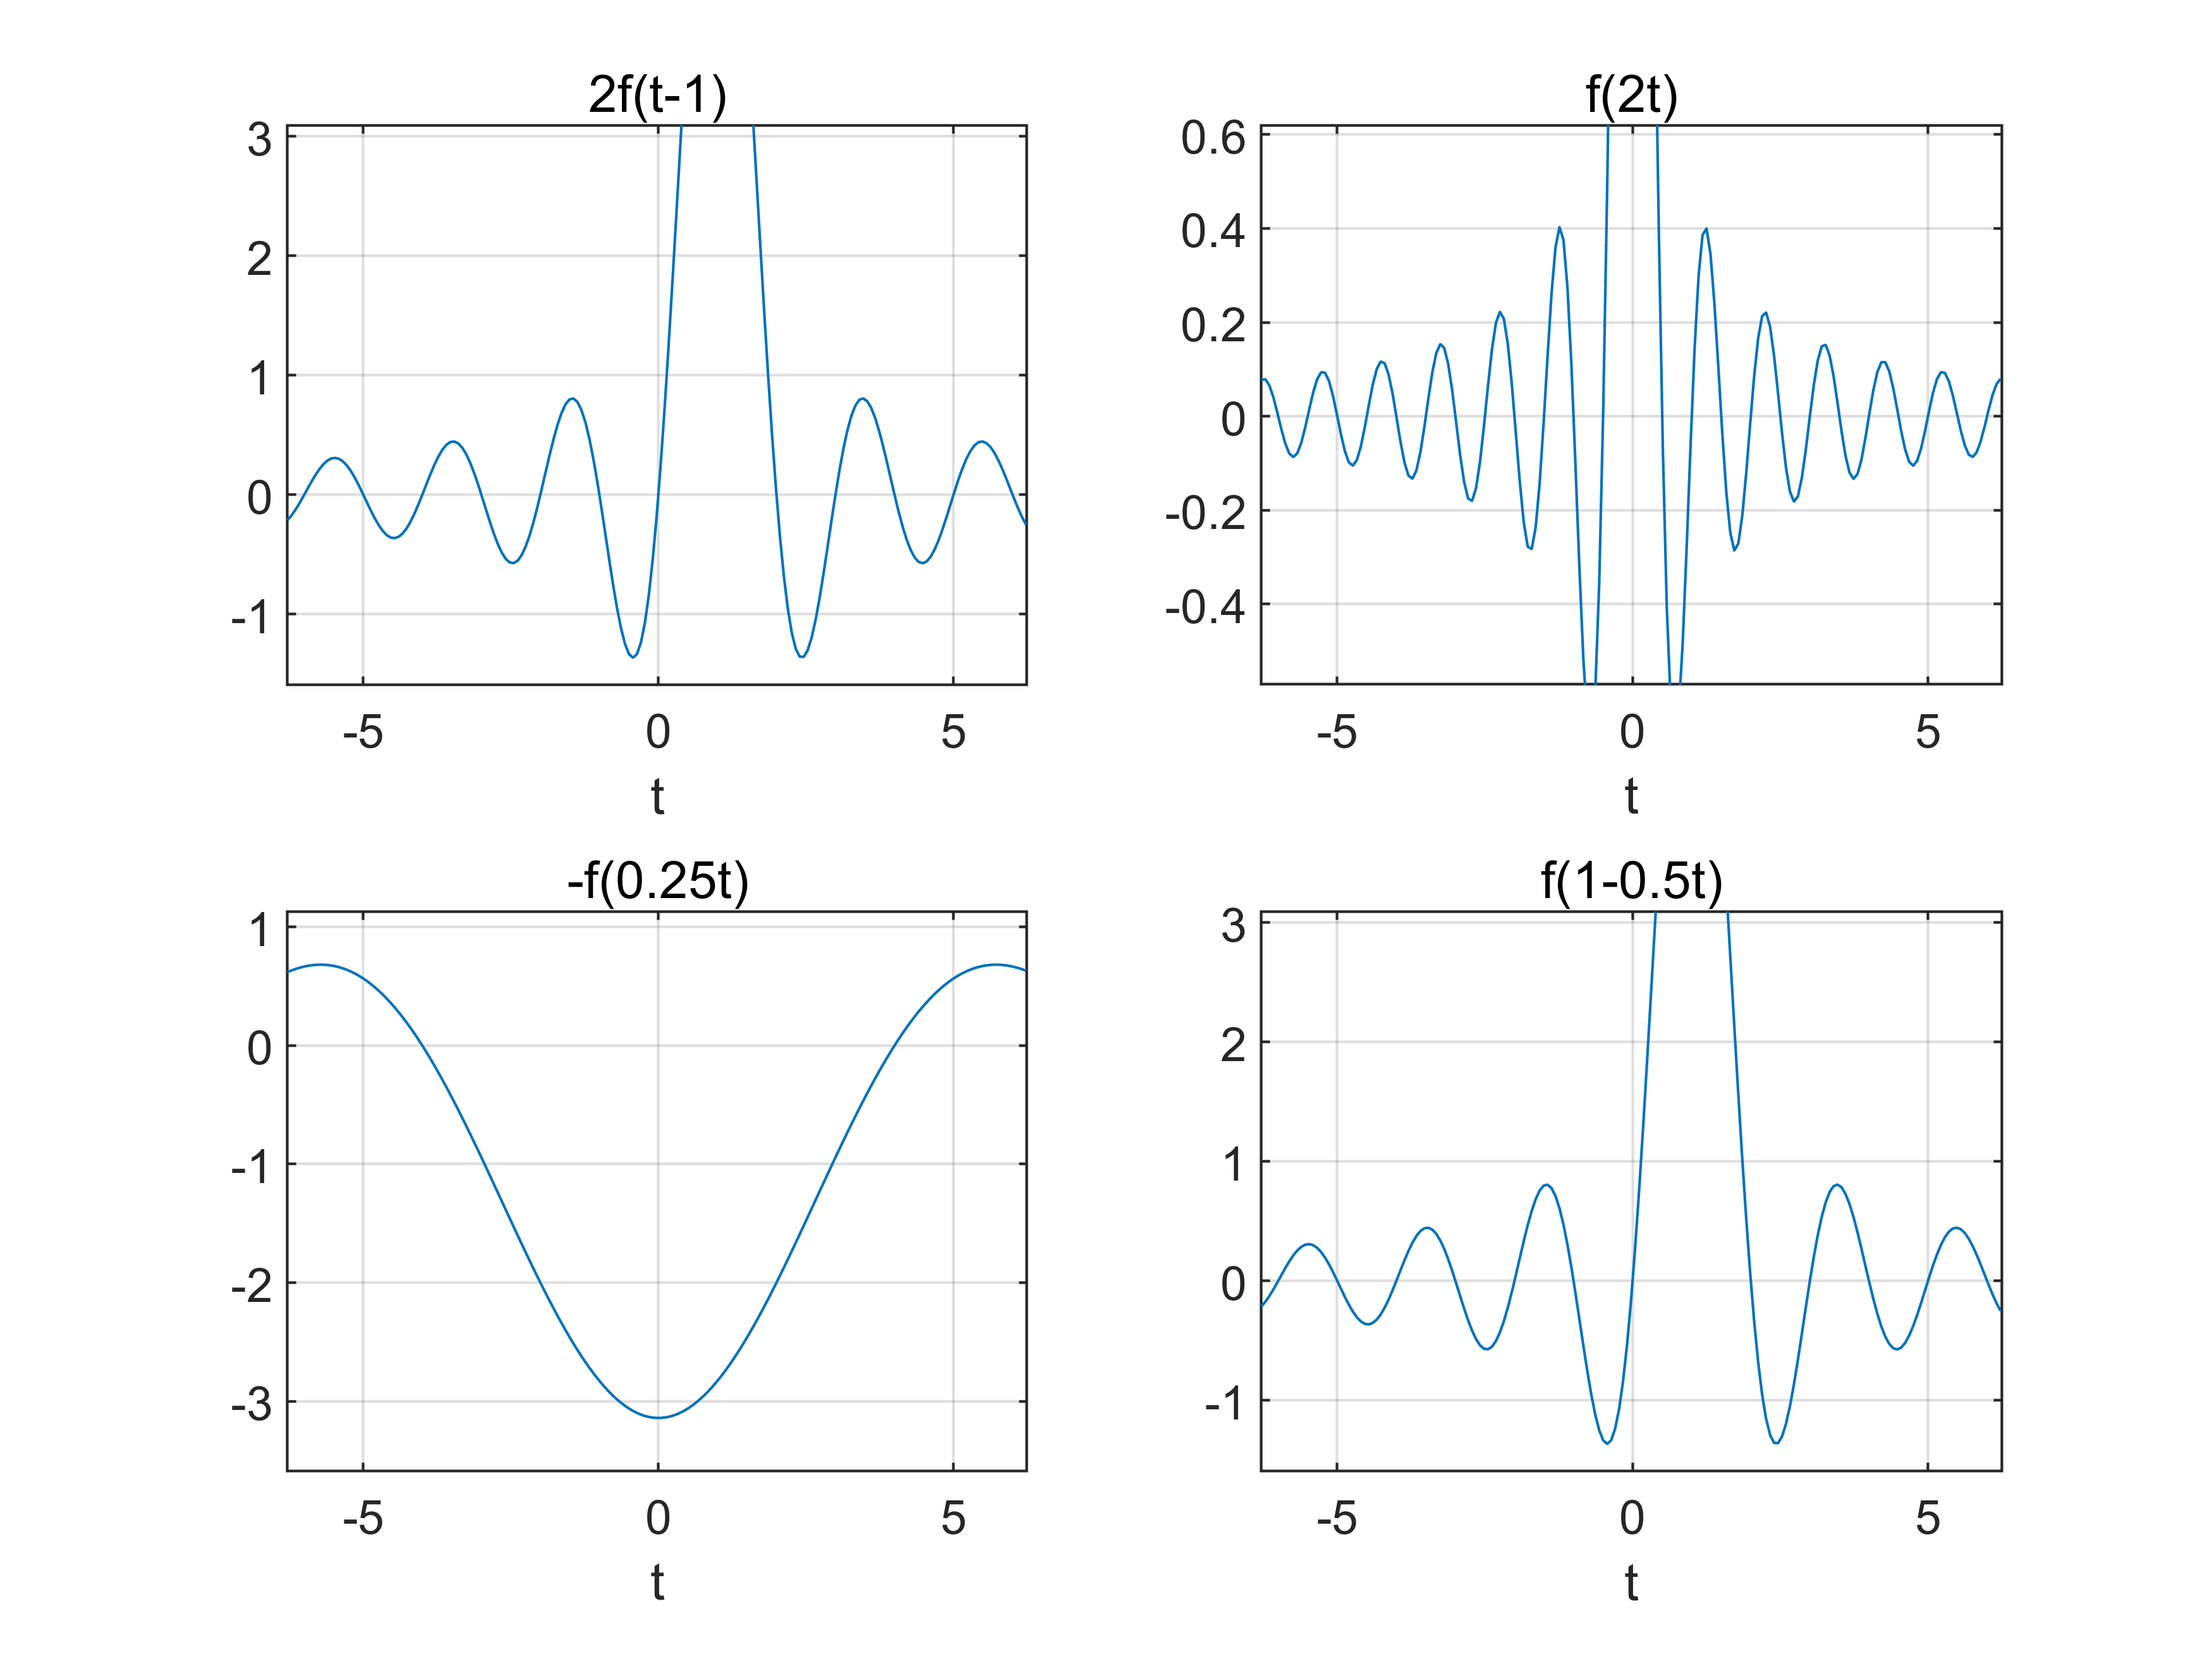
\includegraphics[scale=0.9]{2.png}\\
\end{document}